\documentclass[main.tex]{subfiles}

\begin{document} 
\textit{The work in this chapter is based on \cite{Bourton:2017pee}.}

\section{Introduction}
Using the localisation procedure outlined in Section \ref{sec:intronekpart} Nekrasov was able to verify the results of Seiberg \& Witten \cite{Seiberg:1994rs,Seiberg:1994aj} from a purely field theoretic perspective and derive the instanton partition function for $\mathcal{N}=2$ gauge theories by performing the integration over instanton moduli space \cite{Nekrasov:2003rj,Nekrasov:2002qd}. From his work it is possible to write down the instanton partition functions for general Lagrangian theories in class $\mathcal{S}$. 

While the localisation procedure used in Nekrasov's computation relies on $\mathcal{N}=2$ supersymmetry (in order to preserve a supersymmetry via topological twisting on $\Omega$-background) one can also consider the analagous quantity for theories with less (or no) supersymmetry. Indeed, the idea of expanding the path integral around instanton configurations and integrating over instanton moduli space is an idea that dates back to `t Hooft \cite{PhysRevD.14.3432}. However, for non-supersymmetric theories the fluctations around the instanton background at strong coupling are very hard to perform; while for supersymmetric theories the fluctations cancel. See also \cite{Tachikawa:2014dja,Dorey:2002ik} for reviews. 

In this chapter we will compute the instanton partition functions and verify the proposal of \cite{Mitev:2017jqj} for a subset of class $\mathcal{S}_k$ theories with a Lagrangian description; we take the compactification surface $\mathcal{C}$ to be either an $\ell$-punctured torus $T^2\setminus\{p_1,\dots,p_\ell\}$ or an $\ell+2$-punctured sphere $\mathbb{CP}^1\setminus\{p_1,\dots,p_{\ell+2}\}$. We discussed these theories in detail in Section \ref{sec:introSk}. These theories are conformal and have weakly coupled Lagrangian descriptions in terms of toroidal  or cylindrical $\N=1$ quiver theories. 

Because of their orbifold constructions class $\mathcal{S}_k$ theories suggest an ideal starting point to begin to look for exact results and 2d/4d relations in 4d $\mathcal{N}=1$ theories which, so far, have been largely unexplored. Often the orbifolded daughter theory possesses many similarities with their mother theory \cite{Bershadsky:1998mb,Bershadsky:1998cb}.


We engineer the toroidal $\N=1$ quiver theories of class $\mathcal{S}_k$ in Type-IIB string theory as $\mathbb{Z}_\ell \times \mathbb{Z}_k$ orbifolds of D$3$-branes; as in Section \ref{sec:quivers}.
We can then study the dynamics of $K$ instantons on the D$p$-branes via
the correspondence between the ADHM construction \cite{Atiyah:1978ri} and D$(-1)$-branes within D$3$-branes; explained in Section \ref{intro:secadhmstring}. The instanton moduli space on D$3$-branes is isomorphic to the Higgs branch of the theory on D$(-1)$-branes.
The partition function of the supersymmetric matrix model theory on the worldvolume of $K$ D$(-1)$-branes is then equal to the $K$ instanton partition function of the corresponding  class $\mathcal{S}_k$ theory.

Instantons of orbifold daughters of $\mathcal{N}=4$ SYM were intensively studied in the early days of $AdS$/CFT \cite{Dorey:1999pd,Hollowood:1999bm,Billo:2002hm,Billo:2006jm,Billo:2007py,Argurio:2007vqa,Billo:2008sp} and recent computations in theories with eight or more supercharges in various dimensions \cite{Hwang:2014uwa,Kim:2011mv,Kim:2017xan,Haghighat:2013tka,Haghighat:2013gba} have been possible due to significant improvement of the old techniques.

Using T-duality on the setup of D$3$-branes in the presence of a  $\mathbb{Z}_\ell \times \mathbb{Z}_k$ orbifold singularity we land on D$5$-branes in the presence of a $\mathbb{Z}_\ell \times \mathbb{Z}_k$ orbifold which engineers a 6d (elliptic) uplift of the 4d theories we are interested in.
The matrix model describing pointlike instantons of the 4d theory living on D$3$-branes is lifted to a 2d gauge theory, the superconformal index of which computes the instanton partition function of the corresponding 6d gauge theory on $T^2$, living on the worldvolume of the D$5$-branes. 
The 2d superconformal calculation is very well studied \cite{Putrov:2015jpa,Gadde:2013ftv,Gadde:2014ppa,Gadde:2013lxa,Nakayama:2011pa,Cordova:2017ohl}. 
Taking the 4d limit of the 6d instanton partition function
we obtain the instanton partition function of the 4d class $\mathcal{S}_k$ theory. 

\section{Brane Setup}
\begin{table}[h!]
\centering
\begin{tabular}{ |c |c| c| c| c| c| c| c| c| c| c| }
\hline
   & $X^1$ & $X^2$ & $X^3$ & $X^4$ & $X^5$ & $X^6$ & $X^7$ & $X^8$ & $X^9$& $X^{10}$\\\hline 
 $N$ D$5$ & -- & -- & -- & -- & -- & -- & $\cdot$ & $\cdot$ & $\cdot$ & $\cdot$\\ \hline
 $A_{\ell-1}$ & $\cdot$ & $\cdot$ & $\cdot$ & $\cdot$ & $\cdot$ & $\cdot$ & $\times$ &$\times$ & $\times$ & $\times$\\ \hline
 $A_{k-1}$ & $\cdot$ & $\cdot$ & $\cdot$ & $\cdot$ & $\times$ & $\times$ & $\cdot$ & $\times$ & $\times$ & $\cdot$\\ \hline
 \hline
 $K$ D$1$ & $\cdot$ & $\cdot$ & $\cdot$ & $\cdot$ & -- & -- & $\cdot$ & $\cdot$ & $\cdot$ & $\cdot$ \\\hline
\end{tabular}
\caption{\it Type IIB setup engineering a 6d uplift of the 4d $\mathcal{N}=1$ theories.}
\label{table:D5D1}
\end{table}
In this paper our primary interest will be that of the theory living on the D$(-1)$/D$0$-branes in the setups of Tables \ref{table:D3D-1} and \ref{table:D4D01}. In both cases these are supersymmetric matrix models invariant under at least two supercharges. We could choose to work directly with these matrix models, however we find it more convenient to work instead with the two dimensional uplift of those matrix models. Hence, we instead work with the brane setup of Table \ref{table:D5D1}. Before performing the T-duality we also assume that $X^5$ may be safely decompactified such that it parametrises a space with the topology of $\mathbb{R}$. The T-duality may again be performed by replacing $A_{\ell-1}$ with TN$_{\ell}$ , we then T-dualise along the TN$_{\ell}$ circle, landing us on the setup of Table \ref{table:D5D1} .
The $Spin(6)_{R}$ $R$-symmetry group has been broken to a subgroup $U(1)_{56}\times Spin(4)_R$ which acts by rotations along $\mathbb{R}^2$, $\mathbb{R}^4$ parametrised by $X^5,X^6$ and $X^7,X^8,X^9,X^{10}$ respectively. The $\mathbb{Z}_{\ell}$ orbifold further breaks the $Spin(4)_R$ $R$-symmetry group down to a subgroup $SU(2)_{R}$ corresponding to the isometry group of TN$_{\ell}$, while, the $\mathbb{Z}_k$ orbifold breaks the $U(1)_{56}\times SU(2)_R$ down to the maximal torus of $SU(2)_R$.


\begin{figure}[h]\label{fig:sub}
%\centering
\begin{subfigure}[c]{0.5\linewidth}
\centering
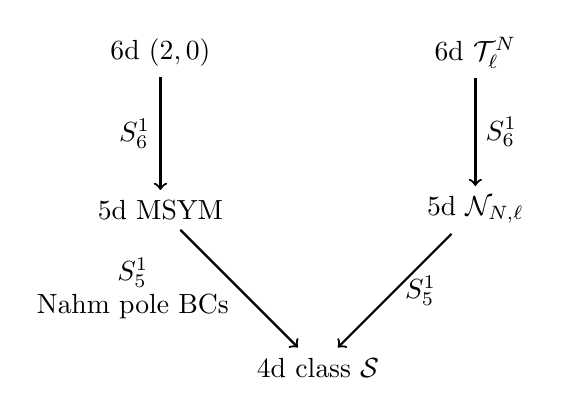
\begin{tikzpicture}[thick,scale=1]
\node (A1) at (-2,4) {6d $(2,0)$}; 
\node [align=center] (A2) at (-2,2) {5d MSYM}; 
\node (B1) at (2,4) {6d $\mathcal{T}^N_{\ell}$}; 
\node (B2) at (2,2) {5d $\mathcal{N}_{N,\ell}$}; 
\node (C) at (0,0) {4d class $\mathcal{S}$}; 

\draw[->] (A1) -- (A2) node[midway,left] {$\mathbb{S}^1_6$};
\draw[->] (B1) -- (B2) node[midway,right] {$\mathbb{S}^1_6$};
\draw[->] (B2) -- (C) node[midway,right] {$\mathbb{S}^1_5$};
\draw[->] (A2) -- (C) node[midway,left,align=center] {$\mathbb{S}^1_5$\\Nahm pole BCs};
\end{tikzpicture}
%\hfill
\caption{\label{ComplactificationsWithZell}}
\end{subfigure}
\hspace*{\fill}
\begin{subfigure}[c]{0.5\linewidth}
\centering
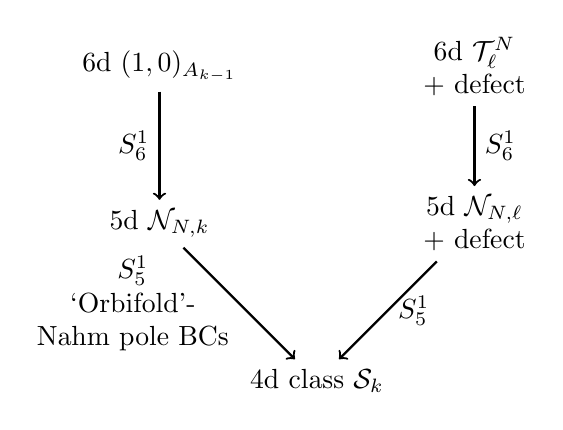
\begin{tikzpicture}[thick, scale=1.0]
\node (A1) at (-2,4) {6d $(1,0)_{A_{k-1}}$}; 
\node (A2) at (-2,2) {5d  $\mathcal{N}_{N,k}$}; 
\node[align=center] (B1) at (2,4) {6d $\mathcal{T}^{N}_{\ell}$\\ + defect}; 
\node[align=center] (B2) at (2,2) {5d $\mathcal{N}_{ N,\ell}$\\ + defect}; 
\node (C) at (0,0) {4d class $\mathcal{S}_k$}; 

\draw[->] (A1) -- (A2) node[midway,left] {$\mathbb{S}^1_6$};
\draw[->] (B1) -- (B2) node[midway,right] {$\mathbb{S}^1_6$};
\draw[->] (B2) -- (C) node[midway,right] {$\mathbb{S}^1_5$};
\draw[->] (A2) -- (C) node[midway,left,align=center] {$\mathbb{S}^1_5$\\`Orbifold'- \\Nahm pole BCs};
\end{tikzpicture}
\caption{\label{ComplactificationsWithZellZk}}
\end{subfigure}
\caption{Left: \it Schematic overview for $k=1$ of two alternate ways to obtain the 4d $\N=2$ $\tilde{A}_{\ell-1}$ circular quivers with $SU(N)^\ell$ gauge group in class $\mathcal{S}$ from compactifications of 6d theories. \normalfont Right: \it A schematic overview of the $k>1$ generalisations of 6d compactifications. The resulting 4d SCFTs are $\N=1$ $\tilde{A}_{\ell-1}\times \tilde{A}_{k-1}$ torodial quivers in class $\mathcal{S}_k$ with gauge group $SU(N)^{\ell k}$.}
\end{figure}

We can discuss the 6d theory on D5-branes. Let us begin with the $k=1$ case. Without the $A_{\ell-1}$ transverse orbifold the theory on $N$ D5-branes is simply the 6d $\mathcal{N}=(1,1)$ SYM theory. Upon performing the $\mathbb{Z}_{\ell}$ quotient we have a 6d $\mathcal{N}=(1,0)$ quiver theory of vector multiplets with bifundamental hypermultiplets, which we will call $\mathcal{T}^N_{\ell}$, see Figure \ref{fig:5dNNl}. 
\begin{figure}
\centering
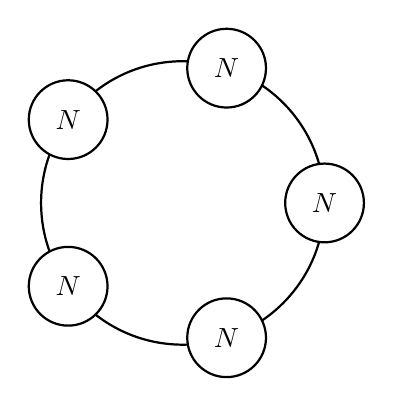
\begin{tikzpicture}[square/.style={regular polygon,regular polygon sides=4},thick,inner sep=0.1em]
   \newdimen\R
   \R=1.8cm
   \draw (0,0) circle (\R);
   \foreach \x/\l/\p in
     { 72/{3},
      144/{2},
      216/{1},
      288/{6},
      360/{4}
     }
     \node[circle,draw,minimum size=1.0cm,fill=white] at (\x:\R) {$N$};
\end{tikzpicture}
\caption{\it 6d circular (necklace) quiver $\mathcal{T}^N_{\ell}$ for $\ell=5$. Circular nodes denote $\mathcal{N}=(1,0)$ vector multiplets and solid lines connecting them denote bifundamental $\mathcal{N}=(1,0)$ hypermultiplets. $\mathbb{S}^1/T^2$ reduction of $\mathcal{T}^N_{\ell}$ results in the 5d/4d circular $\tilde{A}_{\ell-1}$ affine quiver theories.}
\label{fig:5dNNl}
\end{figure}
Compactifying on $\mathbb{S}^1_6$ gives 5d $\N=1$ circular quivers $\mathcal{N}_{N,\ell}$ with $\ell$ nodes denoting $SU(N)$ gauge groups and $\ell$ links denoting bifundamental hypermultiplets. Further compactification on $\mathbb{S}^1_5$ results in 4d $\N=2$ $\tilde{A}_{\ell-1}$ circular quiver theories. The $\tilde{A}_{\ell-1}$ theory may also be realised via the well known class $\mathcal{S}$ construction obtained by compactifying the $A_{N-1}$ $(2,0)$ theory on the $\ell$ punctured torus with certain $\frac{1}{2}$-BPS Nahm pole boundary conditions specified at the punctures \cite{Chacaltana:2012zy,Tsimpis:1998zh,Xie:2013gma}, see Figure \ref{ComplactificationsWithZell}.
  
When $k>1$ the resulting 6d theory corresponds to $\mathcal{T}^{N}_{\ell}$ in the presence of 
a codimension-two Gukov-Witten \cite{Gukov:2006jk,Gukov:2008sn} surface operator % of type $\mathbb{L}$,
 associated to $\ell$ copies of the partition 
\begin{equation}\label{eqn:levipartition}
kN=N_1+\dots+N_k=N+\dots+N
\end{equation}
for the factors of $SU\left(kN\right)^{\ell}$. Finally, KK reducing along the circle leads to the 5d $\N=1$ circular/necklace quiver gauge theory $\mathcal{N}_{N,\ell}$ on $\mathbb{R}^4\times \mathbb{S}^1_5$ in the presence of the defect along the circle (see Figure \ref{ComplactificationsWithZellZk}). Analogously, there is also the class $\mathcal{S}_k$ construction obtained by compactification of the $(1,0)_{A_{k-1}}$ SCFT associated to $N$ M5-branes on transverse $A_{k-1}$ singularity on a torus with $\ell$ punctures with `orbifold' Nahm pole boundary conditions specified at each puncture \cite{Gaiotto:2015usa,Heckman:2016xdl,Hassler:2017arf}.

\subsection{Supersymmetry of the D1/D5 System}
Type IIB string theory has $32$ supersymmetries parametrised by two $32$ component spinors $\epsilon_L$ , $\epsilon_R$ of positive chirality $\Gamma^{11}\mathcal{\epsilon}_{L/R}=+\mathcal{\epsilon}_{L/R}$ where $\Gamma^{11}=\Gamma^1\dots\Gamma^{10}$ and $\Gamma^M$ are the $32\times32$ Gamma matrices.
The D$5$/D$1$ system preserves $1/4$ of the $32$ supersymmetries. Between them they preserve only those supersymmetries of the form
\begin{equation}
\epsilon_L=\Gamma^1\Gamma^2\Gamma^3\Gamma^4\Gamma^5\Gamma^6\epsilon_R\,,\quad \epsilon_L=\sigma\Gamma^5\Gamma^6\epsilon_R\,,
\end{equation} 
with $\sigma=\pm1$ corresponding to whether we choose to insert D$1$- or anti-D$1$-branes. The theory living on the (anti-)D$1$-branes then possesses $(p,q)$ supersymmetry with $p+q=32/4=8$. By choosing an explicit representation for the Gamma matrices it can be shown that $p=q=4$ and that the preserved supercharges are 
\begin{align}
&\Qtwo^{\alpha a}_{+},\quad \Qtwo^{\alpha \dot a}_{-},\quad \text{if $\sigma=+1$}\\
&\widetilde{\Qtwo}^{\dot\alpha\dot a}_{+},\quad\widetilde{\Qtwo}^{\dot\alpha a}_{-},\quad \text{if $\sigma=-1$}
\end{align}
where $a,\dot a=1,2$ are indices of $Spin(4)\iso SU(2)_{a}\times SU(2)_{\dot a}$ and the subscript $\pm$ on fermions denotes the $\pm\frac{1}{2}$ representation under the $U(1)_{56}$ which acts as the Lorentz group of the D$1$-brane worldvolume theory.

The $SU(2)_{a}\times SU(2)_{\dot a}$ rotates the two planes of the $\mathbb{C}^2$ parametrised by $z_2,z_3$ into one another. The Cartans of $\mathfrak{su}(2)_{a},\mathfrak{su}(2)_{\dot a}$ $j_L,j_R$ may be expressed in terms of the generators $J_{710}$ and $J_{89}$ of $U(1)$ rotations in their respective planes as
\begin{equation}
\label{eq:RsymmetryRotations}
j_L=\frac{1}{2}\left(J_{710}-J_{89}\right)\,,\quad j_R=\frac{1}{2}\left(J_{710}+J_{89}\right)\,,
\end{equation}
which are defined such that lower $a=1,2$ have $j_L=+\frac{1}{2},-\frac{1}{2}$ and lower $\dot{a}=\dot1,\dot2$ have $j_R=+\frac{1}{2},-\frac{1}{2}$. Hence the $\Gamma$ action on the supercharges is 
\begin{align}
\label{Qorbifold1}
&\Gamma:\left(\Qtwo^{\alpha a}_{+},\Qtwo^{\alpha \dot a}_{-}\right)\mapsto\omega_{\ell}^{2j_L}\omega_k^{J_{56}+j_L-j_R}\left(\Qtwo^{\alpha a}_{+},\Qtwo^{\alpha \dot a}_{-}\right)\,,\\\
\label{Qorbifold2}
&\Gamma:\left(\widetilde{\Qtwo}^{\dot\alpha\dot a}_{+},\widetilde{\Qtwo}^{\dot\alpha a}_{-}\right)\mapsto\omega_{\ell}^{2j_L}\omega_k^{J_{56}+j_L-j_R}\left(\widetilde{\Qtwo}^{\dot\alpha\dot a}_{+},\widetilde{\Qtwo}^{\dot\alpha a}_{-}\right).
\end{align}
Hence, the supercharges which survive the orbifold action are $\Qtwo^{\alpha\dot1}_{-}$ for $\sigma=+1$ or $\widetilde{\Qtwo}^{\dot\alpha\dot2}_{+}$ for $\sigma=-1$.
We will use one of them to compute the superconformal index in the next section.

\section{Instantons for 4d \texorpdfstring{$\N=2^*$}{N=2*} SYM}\label{Sec:2star}
In this section we warm up for our main calculation that we perform in the next section by reproducing the well known instanton partition function of $\mathcal{N}=2^*$ via a 2d superconformal index calculation.
We parameterise our partition function and use a supercharge that survives the orbifold projection \eqref{Qorbifold1} \eqref{Qorbifold2} so that we are well prepared for the next section.

As discussed in Section \ref{Chap:AppInstADHM}, there is a correspondence between the ADHM construction of instantons \cite{Atiyah:1978ri} and D$(p-4)$-branes \cite{Douglas:1996uz,Douglas:1995bn,Witten:1994tz,Tong:2005un,Polchinski:1996na}. Since the class $\mathcal{S}_k$ gauge theories of interest in this chapter may be realised within Type-II string theory as a theory living on the worldvolume of D$p$-branes we may use this correspondence to derive its ADHM construction.
The case that interests us is the case $p=5$, i.e. D$5$-branes on $\mathbb{R}^4\times T^2$, thus we have to compute the partition function of the 2d gauge theory living on the world volume D$1$-branes wrapping a $T^2$. This partition function is the 2d superconformal index a.k.a. flavoured elliptic genus.

\subsection{D1 Worldvolume Theory}
Before discussing the supersymmetric index we must first discuss the worldvolume theory living on the D$1$-branes in the low energy limit in the presence of the D5s.
\paragraph{D1-D1}
The theory arising from quantising open strings stretching between $K$ parallel and coincident D$p$-branes is given by $p+1$ dimensional Yang-Mills theory with $16$ supercharges, for $p=1$ that is the well known $\N=(8,8)$ SYM theory. In terms of multiplets under the $\N=(4,4)$ subalgebra given by $\widetilde{\Qtwo}_{+}^{\dot\alpha \dot a},\widetilde{\Qtwo}_{-}^{\dot\alpha a}$ they form a $\N=(4,4)$ vector multiplet $V$ and hypermultiplet $H$, which can be thought of as the reduction to 2d of a 4d $\N=2$ vector multiplet and hypermultiplet respectively. $V$ contains a 2d gauge field $A_{\pm}$, four scalars degrees of freedom $Y_{a\dot a}$, right moving fermions $\overline{\lambda}^{\dot\alpha a}_{+}$ and left moving fermions $\overline{\xi}_{-}^{\dot\alpha\dot a}$. $H$ contains scalars $X_{\alpha\dot\alpha}$, right moving fermions $\xi_{+}^{\alpha\dot a}$ and left moving fermions $\lambda^{\alpha a}_{-}$.

\paragraph{D1-D5}
Open D$1$-D$5$ strings preserve $\N=(4,4)$ supersymmetry and gives rise to a $\N=(4,4)$ hypermultiplet $U$ in the bifundamental representation of $U(K)\times SU(N)$. $U$ contains two complex scalars $\phi^{\dot\alpha}$ and their conjugates $\phi^{\dagger}_{\dot\alpha}$, and fermions $\chi^{\dot a}_{+}$, $\psi^{a}_{-}$ plus their conjugates $\chi^{\dagger}_{+\dot{a}}$, $\psi^{\dagger}_{-a}$.
\begin{figure}
\centering
\begin{tikzpicture}[square/.style={regular polygon,regular polygon sides=4},thick,scale=0.9]
 \node(G) at (0,0)[circle,draw,minimum size=1cm]{$K$};
 \node(F) at (0,2)[square,draw]{$N$};
 \draw (F.-90)--(G.90);
 \draw (G) to [out=240,in=300,looseness=6](G);
\end{tikzpicture}
\caption{\it The $\N=(4,4)$ 2d quiver of the gauge theory on $K$ D1-branes in the presence of $N$ D5-branes.}
\label{fig:D1quiver}
\end{figure}
Finally, the field content may be conveniently summarised in the quiver diagram of Figure \ref{fig:D1quiver}. There, using $\N=(4,4)$ notation, solid lines denote hypermultiplets, while the circular node denotes the $U(K)$ vector multiplet.

\paragraph{ADHM Equations}
We can easily obtain the BPS equations on the Higgs-branch of this system. As we elucidated in Section \ref{Chap:AppInstADHM} these translate to the ADHM equations \eqref{eqn:BPSADHM} $F=\mu_{\mathbb{C}}=0$, $D=\mu_{\mathbb{R}}-\zeta\mathbb{I}_K=0$. The Higgs branch is reached by setting $Y_{a\dot a}=0$.

Before the $\mathbb{Z}_k\times\mathbb{Z}_{\ell}$ orbifolding the non-zero $F$- and $D$-term equations on the Higgs-Branch read
\begin{gather}
D+\zeta\mathbb{I}_K=\mu_{\mathbb{R}}=JJ^{\dagger}-I^{\dagger}I+[B_1,B_1^{\dagger}]+[B_2,B_2^{\dagger}]=\zeta\mathbb{I}_{K}\,,\\
F=\mu_{\mathbb{C}}=JI+[B_1,B_2]=0\,.
\end{gather}
where $J=\phi^{\dot1}$, $I=\overline{\phi}^{\dot1}$, $B_1=X^{1\dot1}$ and $B_2=X^{2\dot1}$. The orbifolding acts rather simply on those fields since they all have $j_L=J_{56}=0$. The only non-trivial action is due to the gauge \eqref{eqn:orbifoldactionUK} and flavour \eqref{eqn:orbifoldactionSUN} holonomies. We have
\begin{gather}
D_{ni}+\zeta\mathbb{I}_{K_{ni}}=\mu^{(ni)}_{\mathbb{R}}=J_{ni}J^{\dagger}_{ni}-I^{\dagger}_{ni}I_{ni}+[B_{1,ni},B^{\dagger}_{1,ni}]+[B_{2,ni},B^{\dagger}_{2,ni}]\,,\\
F_{ni}=\mu^{(ni)}_{\mathbb{C}}=I_{ni}J_{ni}+[B_{1,ni},B_{2,ni}]\,.
\end{gather}
The Higgs-branch, or equivalently the $\{K_{11},\dots,K_{\ell k}\}$-instanton moduli space is then
\begin{equation}\label{eqn:ADHMSigmaModel1}
\begin{aligned}
&\mathbf{M}_{\{K_{ni}\}}\iso\mathbf{HB}\\
&=\left\{B_{1,ni}\,,B_{2,ni}\,,I_{ni}\,,J_{ni}\,|\,\mu^{(ni)}_{\mathbb{R}}=\zeta\mathbb{I}_{K_{ni}}\,,\mu^{(ni)}_{\mathbb{C}}=0\right\}/\left(\prod_{i,n}U(K_{ni})\right)\,.
\end{aligned}
\end{equation}
\subsection{Elliptic Genus Computation}
We now turn to the computation of the supersymmetric index a.k.a flavoured elliptic genus partition function for our $\N=(4,4)$ theory.
The supersymmetric index can be understood as the Witten index of the theory quantised on $\mathbb{S}^1\times \mathbb{R}$ refined by fugacities which keep track of further relevant quantum numbers and it is independent of the coupling constants of the theory.
 Since our theory admits a free field limit, computing the index is equivalent to enumerating all gauge invariant operators of the theory on $\mathbb{R}^2$ \cite{Putrov:2015jpa,Gadde:2013wq,Gadde:2013ftv,Gadde:2014ppa,Gadde:2013lxa,Nakayama:2011pa,Cordova:2017ohl}. 
For theories with a Lagrangian description the index  can also be obtained using localisation techniques \cite{Benini:2013nda,Benini:2013xpa} and explicitly performing the path integral of the 2d theory on $T^2$, however for simplicity we will follow the former approach.

We also choose to view our $\N=(4,4)$ theory as an $\N=(0,2)$ theory with additional flavour symmetry. We choose the $\N=(0,2)$ supercharges to be 
\begin{equation}\label{eqn:02susycharges}
\Qtwo:=\widetilde{\Qtwo}_{+}^{\dot2\dot1}, \quad\widetilde{\Qtwo}:=\widetilde{\Qtwo}_{+}^{\dot1\dot2}\,.
\end{equation} 
2d $\N=(0,2)$ theories have a single right moving $U(1)_{\mathfrak{R}}$ $R$-symmetry. The $\N=(0,2)$ IR $R$-symmetry for this model was computed in \cite{Tong:2014yna} and it is given by\footnote{Our D$5$/D$1$ setup is precisely that of \cite{Tong:2014yna} with $Q_5^+=N$, $Q_5^-=0$, $R^-=-2j_2$ and $R^+=-2j_R$.}
\begin{equation}
\label{eq:IRrsymmetry}
\mathfrak{R}_{\text{IR}}=-2j_2\,,
\end{equation}
under which $\mathfrak{R}_{\text{IR}}[\Qtwo]=-1$ and $\mathfrak{R}_{\text{IR}}[\widetilde{\Qtwo}]=+1$.
We will compute the index which counts cohomology classes of $\widetilde{\Qtwo}$. Since $\widetilde{\Qtwo}$ and its conjugate $\widetilde{\Qtwo}^{\dagger}=\widetilde{\Stwo}$ commutes with $SU(2)_{\alpha}$ and $SU(2)_{a}$ we may include fugacities $v$ and $w$ for their Cartans. Furthermore, they also commute with the diagonal subgroup $SU(2)_D\subset SU(2)_{\dot\alpha}\times SU(2)_{\dot a}$ hence we also include a fugacity $z$ for its Cartan $j_D=j_2+j_R$.
Recall that\footnote{The Cartans of $\mathfrak{su}(2)_{a}$ and $\mathfrak{su}(2)_{\dot a}$ denoted as $j_L$ and $j_R$ can be written in terms of the generators $J_{710}$ and $J_{89}$ which are the $U(1)$ rotations in the respective planes  \eqref{eq:RsymmetryRotations}.} the Cartans of $\mathfrak{su}(2)_{\alpha},\mathfrak{su}(2)_{\dot\alpha},\mathfrak{su}(2)_{a}$ and $\mathfrak{su}(2)_{\dot a}$  all commute with the orbifold and the fugacities $v,w$ and $z$ that we introduced here will still be meaningful for our calculation in the next section.
 We also include fugacities $x_A$ for the Cartans $f_A$ of $\mathfrak{su}(N)$ and $y_I$ for the Cartans $g_I$ of $\mathfrak{u}(K)$. The index is then defined as
\begin{equation}\label{eqn:2starindex}
Z^{6d}_K(q,v,w,z,x_A)= \Tr(-1)^Fq^{H_-}\overline{q}^{\delta}v^{2j_1}w^{2j_L}z^{2j_2+2j_R}\prod_{A=1}^Nx_A^{f_A}\prod_{I=1}^Ky_{I}^{g_I}
\end{equation}
where $F=F_-+F_+$ is the fermion number and $H_-$, $H_+$ are the left and right moving Hamiltonians, respectively. In Euclidean signature we define $2H_{\pm}=H\mp\iu P$ and $q:=e^{2\pi\iu\tau}$ with $\tau$ the complex structure of the $T^2$ is generated by $\omega\sim \omega+1\sim \omega+\tau$. Explicitly, we will work with the square torus with complex structure $\tau=\iu\beta_6/\beta_5$ with $\beta_5$, $\beta_6$ the radii of the two $\mathbb{S}^1$ factors.
In radial quantisation the conformal map from the plane to the cylinder is $z_1=e^{2\pi\iu \omega}$, where $\omega:=\sigma+\iu t$ and Lorentz transformations $z_1\mapsto e^{\iu\theta}z_1$ are then mapped to translations around the $\mathbb{S}^1$ factor of the cylinder
\begin{equation}\label{lorentz}
\left(\sigma,t\right)\mapsto \left(\sigma+\frac{\theta}{2\pi}, t\right)
\end{equation}
generated by $P=i J_{56}$. 

One of the crucial properties of the quantity \eqref{eqn:2starindex} is that it receives contributions only from those states which satisfy 
\begin{equation}\label{eq:delta}
\delta= \left\{ \widetilde{\Qtwo} , \widetilde{\Stwo} \right\} =H_+-\frac{1}{2}\mathfrak{R}
=0
\end{equation}
where $\mathfrak{R}$ is the $\N=(0,2)$ $R$-symmetry; the index is independent of $\overline{q}$. Furthermore the index \eqref{eqn:2starindex} is also independent of all continuous parameters such as coupling constants and Fayet-Iliopoulos parameters \cite{Witten:1982df,Kinney:2005ej}, hence we can compute the index in the free field limit where it reduces to a counting problem.

In the free field limit we have a $\N=(0,2)$ superconformal theory with  $\mathfrak{Vir}\oplus\overline{\mathfrak{sVir}}_{NS}$ symmetry where $\mathfrak{Vir}$ is the standard $(\N=0)$ left-moving Virasoro algebra generated by $\left\{L_n,c\right\}$, $\overline{\mathfrak{sVir}}_{NS}$ is the $\N=2$ super-Virasoro algebra in the NS sector generated by $\left\{\overline{L}_n,\overline{G}^{\pm}_r,\overline{J}_n,\overline{c}\right\}$ and $n,r+\frac{1}{2}\in\mathbb{Z}$. Our choice of the Neveu-Schwarz basis over the Ramond basis is purely for calculational convenience and the index is independent of this choice up to an overall factor \cite{Cordova:2017ohl}. We will require the following brackets of the $\overline{\mathfrak{sVir}}_{\N=2,NS}$ algebra:
\begin{gather}
\left\{\overline{G}^+_r,\overline{G}^-_s\right\}=\overline{L}_{r+s}+\frac{1}{2}(r-s)\overline{J}_{r+s}+\frac{\overline{c}}{6}\left(r^2-\frac{1}{4}\right)\delta_{r+s,0}\,,\\
\left[\overline{L}_0,\overline{G}^{\pm}_{r}\right]=-r\overline{G}^{\pm}_{r}\,,\quad \left[\overline{J}_0,\overline{G}^{\pm}_{r}\right]=\pm\overline{G}^{\pm}_{r}\,.
\end{gather}
In the free field limit, we identify 
\begin{gather}
H_-=L_0,\quad H_+=\overline{L}_0\,,\quad \mathfrak{R}=\overline{J}_0\,,\\ \Qtwo=\overline{G}^{-}_{-\frac{1}{2}}\,,\quad \Stwo=\overline{G}^{+}_{+\frac{1}{2}},\quad \widetilde{\Qtwo}=\overline{G}^{+}_{-\frac{1}{2}}\,,\quad \widetilde{\Stwo}=\overline{G}^{-}_{+\frac{1}{2}} \, .
\end{gather}
%
Away from the free limit, the theory is not conformal and we have an RG flow from the free UV fixed point to an IR fixed point. This IR fixed point is expected to be precisely the ADHM sigma model with target space the instanton moduli space \eqref{eqn:ADHMSigmaModel1}. The $R$-charge assignments generally change along RG flow. Nonetheless, the index is RG invariant and we can evaluate the index at the IR fixed point by using the non-anomalous $R$-symmetry assignment in the IR which, in our case, is \eqref{eq:IRrsymmetry}.

At the UV fixed point the shortening condition  \eqref{eq:delta} can be written as
\begin{equation}\label{eqn:bpscondition}
\delta=\left\{\overline{G}^+_{-\frac{1}{2}},\overline{G}^-_{+\frac{1}{2}}\right\}=\overline{L}_{0}-\frac{1}{2}\overline{J}_{0}=0\,.
\end{equation}
and the states contributing to the index must have $\overline{J}_0=2\overline{L}_0$ in the UV. The IR R-symmetry \eqref{eq:IRrsymmetry} is then taken into account by shifting $q^{L_0}\to q^{L_0-\overline{L}_0+\frac{1}{2}\mathfrak{R}_\text{IR}}$ in the index.

\subsubsection{Letter Counting}
As stressed earlier the index may be computed in the free field limit. This is done by identifying all `letters' with $\delta=0$. The single letter partition functions for the $\N=(4,4)$ multiplets may be easily read off from Tables \ref{tab:Vletters}, \ref{tab:Hletters}, \ref{tab:Uletters} in Appendix \ref{App:EllipticGenus1}. They are given by
\begin{equation}
i_V(q,w,z,y_I)=\left[\frac{\left(w+w^{-1}\right)\left(z+qz^{-1}\right)-qz^{-2}-z^2-2q}{1-q}\right]\sum_{I,J=1}^Ky_Iy_J^{-1}\,,\label{eqn:letterfV}
\end{equation}
\begin{equation}
i_H(q,v,w,z,y_I)=\left[\frac{q^{\frac{1}{2}}\left(v+v^{-1}\right)\left(z+z^{-1}-w^{-1}-w\right)}{1-q}\right]\sum_{I,J=1}^Ky_Iy_J^{-1}\,,\label{eqn:letterfH}
\end{equation}
\begin{equation}
i_U(q,w,z,x_A,y_I)=\left[\frac{q^{\frac{1}{2}}\left(z+z^{-1}-w^{-1}-w\right)}{1-q}\right]\sum_{I=1}^K\sum_{A=1}^N\left(\frac{y_I}{x_A}+\frac{x_A}{y_I}\right)\label{eqn:letterfU}\,.
\end{equation}
The full index is then by enumerating all possible `words' and then projecting onto gauge singlets by integrating over the Haar measure $d\mu_G$ of the $G=U(K)$ gauge group, given in \eqref{eqn:schurmeasure}. The full index is then given by
\begin{equation}
Z^{6d}_K(q,v,w,z,x_A)=\oint d\mu_{U(K)} \,Z^{(0)}\prod_{P=V,H,U}Z_{P}
\end{equation}
where $Z^{(0)}$ is the Casimir contribution which may, apriori, depend on all fugacities. It is given by \cite{Benini:2011nc,Kim:2009wb,Imamura:2011su,Rastelli:2016tbz,Bobev:2015kza,Assel:2015nca,Ardehali:2015bla,Kim:2012ava}
\begin{equation}\label{eqn:casimir}
Z^{(0)}\equiv Z^{(0)}(q,v,w,z)=q^{\frac{1}{2}E_{\text{Casimir}}},\quad E_{\text{Casimir}}=\substack{\text{Finite}\\q\to1}\left[\sum_{P}\frac{\partial i_{P}}{\partial\log q}\right]\,.
\end{equation}
and
\begin{equation}\label{eqn:singpartfunction}
Z_{P}\equiv Z_{P}(q,v,w,z,x_A,y_I):=\PE\left[i_{P}(q,v,w,z,x_A,y_I)\right]\,,
\end{equation}
where $\PE$ denotes the Plethystic exponential; defined in \eqref{eqn:PE} and $i_{P}$ are the single letter partition functions \eqref{eqn:letterfV}, \eqref{eqn:letterfH} and \eqref{eqn:letterfU}. Explicitly:
\begin{equation}
Z_V(q,w,z,y_I)=\prod_{I,J=1}^K\frac{\left(q\frac{y_I}{y_J};q\right)^2\theta\left(qz^{-2}\frac{y_I}{y_J};q\right)}{\theta\left(wz\frac{y_I}{y_J};q\right)\theta\left(qwz^{-1}\frac{y_I}{y_J};q\right)}\,,
\end{equation}
\begin{equation}
Z_H(q,v,w,z,y_I)=\prod_{I,J=1}^K\frac{\theta\left(q^{\frac{1}{2}}vw\frac{y_I}{y_J};q\right)\theta\left(q^{\frac{1}{2}}v^{-1}w\frac{y_I}{y_J};q\right)}{\theta\left(q^{\frac{1}{2}}vz^{-1}\frac{y_I}{y_J};q\right)\theta\left(q^{\frac{1}{2}}v^{-1}z^{-1}\frac{y_I}{y_J};q\right)}\,,
\end{equation}
\begin{equation}
Z_U(q,w,z,x_A,y_I)=\prod_{I=1}^K\prod_{A=1}^N\frac{\theta\left(q^{\frac{1}{2}}w\frac{x_A}{y_I};q\right)\theta\left(q^{\frac{1}{2}}w\frac{y_I}{x_A};q\right)}{\theta\left(q^{\frac{1}{2}}z^{-1}\frac{x_A}{y_I};q\right)\theta\left(q^{\frac{1}{2}}z^{-1}\frac{y_I}{x_A};q\right)}\,,
\end{equation}
where $\theta(x;q)$ and $(x;q)$ are the $q$-theta function and $q$-Pochammer symbol; defined in \eqref{eqn:qtheta} and \eqref{eqn:qPochammer} respectively.
Finally, we conclude that the full index is given by
\begin{equation}\label{eqn:6dpartitionfunctionK}
\begin{aligned}
Z^{6d}_K=&\frac{\left(q;q\right)^{2K}}{K!}\oint_{T(G)}\prod_{I=1}^K\frac{dy_I}{2\pi\iu y_I}\prod_{I=1}^K\prod_{A=1}^N\frac{\theta\left(q^{\frac{1}{2}}w\frac{x_A}{y_I};q\right)\theta\left(q^{\frac{1}{2}}w\frac{y_I}{x_A};q\right)}{\theta\left(q^{\frac{1}{2}}z^{-1}\frac{x_A}{y_I};q\right)\theta\left(q^{\frac{1}{2}}z^{-1}\frac{y_I}{x_A};q\right)}\\
&\times Z^{(0)}\prod_{I,J=1}^K\frac{\theta\left(\frac{y_I}{y_J};q\right)'\theta\left(qz^{-2}\frac{y_I}{y_J};q\right)\theta\left(q^{\frac{1}{2}}vw\frac{y_I}{y_J};q\right)}{\theta\left(wz\frac{y_I}{y_J};q\right)\theta\left(qwz^{-1}\frac{y_I}{y_J};q\right)\theta\left(q^{\frac{1}{2}}vz^{-1}\frac{y_I}{y_J};q\right)}\\
&\times\prod_{I,J=1}^K\frac{\theta\left(q^{\frac{1}{2}}v^{-1}w\frac{y_I}{y_J};q\right)}{\theta\left(q^{\frac{1}{2}}v^{-1}z^{-1}\frac{y_I}{y_J};q\right)}
\end{aligned}
\end{equation}
where the prime means to remove those factors $\theta(1;q)$ and we used the identity $\left(x;q\right)=\left(1-x\right)\left(qx;q\right)$. It also useful to assemble the grand partition function
\begin{equation}\label{eqn:6dpartitionfunction1}
Z^{6d}(q,v,w,z,x_A;\mathbf{q}_{6d}):=\sum_{K\geq0}\mathbf{q}^K_{6d}Z^{6d}_K(q,v,w,z,x_A)
\end{equation}
with $\mathbf{q}_{6d}$ a formal dimensionless parameter. When considering our 6d theory on $\mathbb{R}^4\times \mathbb{S}_5^1\times \mathbb{S}_6^1$ as a 5d theory on $\mathbb{R}^4\times \mathbb{S}_5^1$ dressed by KK modes along  $\mathbb{S}_6^1$ we may regard $\mathbf{q}_{6d}$ as a fugacity for the topological $U(1)$ global symmetry associated to the conserved current $\star_{5d}J=\frac{1}{8\pi^2}\tr F\wedge F$. 

\subsection{The 6d Instanton Partition Function}
The countour integrals \eqref{eqn:6dpartitionfunctionK} may be computed via the Jefferey-Kirwan residue prescription \cite{1993alg.geom..7001J,Benini:2013nda,Benini:2013xpa}. Using \eqref{eqn:residueform}, we can perform the residue prescription. The integrand of \eqref{eqn:6dpartitionfunction1} has simple poles at
\begin{gather}
y_I=y_J\left(zw\right)^{\pm1},\quad y_I=y_J\left(\frac{z}{qw}\right)^{\pm1},\\
y_I=y_J\left(\frac{vz}{q^{1/2}}\right)^{\pm1},\quad y_I=y_J\left(\frac{z}{vq^{1/2}}\right)^{\pm1},\quad y_I=x_A\left(\frac{z}{q^{1/2}}\right)^{\pm1}.\label{eqn:polekeep1}
\end{gather}
As explained in \cite{Kim:2011mv,Kim:2012gu} only residues arising from the poles \eqref{eqn:polekeep1} should be kept. We assume that the $x_A$'s are sufficiently generic and furthermore we close the contour such that we collect residues coming from poles with the positive sign exponents. 
The solutions to \eqref{eqn:polekeep1} may be classified by $N$-coloured Young's diagrams $\vec{\mu}=\left\{\mu_1,\dots,\mu_N\right\}$ with each diagram $\mu_A$ containing $|\mu_A|$ boxes such that $|\vec{\mu}|:=\sum_{A}|\mu_A|=K$. Given a Young's diagram $\mu_A$ a box $s$ is labelled by coordinates $(l,p)$ and the corresponding pole is given by
\begin{equation}
y(s)=x_A\left(\frac{z}{q^{1/2}}\right)^{l+p-1}v^{l-p} \, .
\end{equation}
The residue for a fixed coloured Young diagram is then
\begin{equation}
Z^{6d}_{\vec{\mu}}=Z^{(0)}\prod_{A,B=1}^N\prod_{s\in \mu_A}\frac{\theta\left(q^{-1}zw^{-1}\mathcal{E}_{AB};q\right)\theta\left(zw\mathcal{E}_{AB};q\right)}{\theta\left(\mathcal{E}_{AB};q\right)\theta\left(q^{-1}z^2\mathcal{E}_{AB};q\right)}
\, ,
\end{equation}
where we defined
\begin{equation}
\mathcal{E}_{BA}:=\frac{x_B}{x_A}\left(\frac{vz}{q^{1/2}}\right)^{L_A(s)}\left(\frac{q^{1/2}v}{z}\right)^{A_B(s)+1}
\end{equation}
and where $L_B(s)$ and $A_B(s)$ denote the distance from the box $s$ to the right end and the bottom of the Young diagram $\mu_B$ respectively. $Z^{(0)}=q^{\frac{1}{2}E_{\text{Casimir}}}$ is the Casimir contribution \eqref{eqn:casimir}. To compute it one is forced to specify the $q$-dependence of the fugacities, we hence define  
\begin{equation}\label{eqn:5dvariables}
v:=q^{\frac{\beta_5\epsilon_-}{2\iu\pi}}\,,\quad wq^{\frac{1}{2}}:=q^{\frac{\beta_5m}{\iu\pi}}\,,\quad zq^{-\frac{1}{2}}:=q^{\frac{\beta_5\epsilon_+}{2\iu\pi}}\,,\quad x_A:=q^{\frac{\beta_5a_A}{\iu\pi}}\,,
\end{equation}
where we used the shorthand notation
\begin{equation}
\epsilon_{\pm}:=\epsilon_1\pm\epsilon_2\,.
\end{equation}
$Z^{(0)}$ is then a constant and is given by
\begin{equation}
Z^{(0)}=q^{\frac{\beta_5^2NK}{\pi^2}\left(\frac{\epsilon_+}{2}-m+\frac{\iu\pi}{\beta_5}\right)\left(\frac{\epsilon_+}{2}+m\right)}\,.
\end{equation}
The $K$ instanton partition function \eqref{eqn:6dpartitionfunctionK} is then given by summing over all coloured Young diagrams $\vec{\mu}$.
Hence, equation \eqref{eqn:6dpartitionfunction1} finally reads
\begin{equation}\label{eqn:6dpartitionfunctionyng1}
Z^{6d}:=\sum_{K\geq0}\mathbf{q}_{6d}^K\sum_{\substack{\vec{\mu}\\|\vec{\mu}|=K}}Z_{\vec{\mu}}^{6d}=\sum_{\vec{\mu}}\mathbf{q}^{|\vec{\mu}|}_{6d}Z_{\vec{\mu}}^{6d}\,.
\end{equation}

\subsection{Reduction to Five and Four Dimensions}
Reducing the D5/D1 system on $\mathbb{S}^1_6$ by taking $\beta_6\to0$ results in 5d $\N=2$ SYM with gauge group $SU(N)$ at Chern-Simons level $\kappa=0$. Hence by either taking the 5d limit directly to \eqref{eqn:6dpartitionfunctionyng1} or taking the limit directly the contour integral \eqref{eqn:6dpartitionfunctionK} we expect to obtain the instanton partition function for the 5d theory. Here we take the first approach but we detail the limit of the contour integral expression in Appendix \ref{5dLimitOfUnorbifolded}.

Recall that $q=e^{2\pi\iu\tau}$ and $\tau=\iu\beta_6/\beta_5$ therefore this limit corresponds to taking
\begin{equation}
q\to1\,.
\end{equation}
Further note that, by definition \eqref{eqn:casimir}, 
\begin{equation}
\lim_{q\to1}Z^{(0)}=q^{\frac{1}{2}E_{\text{Casimir}}}=1\,.
\end{equation}
Applying \eqref{eqn:thetafunctionlimit} to \eqref{eqn:6dpartitionfunctionyng1} yields
\begin{align}
&Z^{5d}=\sum_{\vec{\mu}}\mathbf{q}_{5d}^{|\vec{\mu}|}Z_{\vec{\mu}}^{5d}\\
&Z_{\vec{\mu}}^{5d}=\prod_{A,B=1}^N\prod_{s\in \mu_A}\frac{\sinh\beta_5\left(E_{AB}+\frac{\epsilon_+}{2}-m\right)\sinh\beta_5\left(E_{AB}+\frac{\epsilon_+}{2}+m\right)}{\sinh\beta_5\left(E_{AB}\right)\sinh\beta_5\left(E_{AB}+\epsilon_+\right)}\label{5dpartitionfunctionyng}
\end{align}
where we have defined
\begin{equation}
E_{BA}=a_B-a_A+\epsilon_1L_A(s)-\epsilon_2\left(A_B(s)+1\right)\,,
\end{equation}
such that $\mathcal{E}_{AB}=q^{\frac{E_{AB}}{\iu\pi}}$ and we take $\mathbf{q}_{5d}=\lim_{q\to1}\mathbf{q}_{6d}$.
 This reproduces the instanton partition for the mass deformed 5d $\N=2$ theory (a.k.a. $\N=1^*$) on $\mathbb{R}^4\times \mathbb{S}^1_5$ in the $\Omega$-background, which was computed via localisation of the path integral of the ADHM quantum mechanics in e.g. \cite{Hwang:2014uwa,Kim:2011mv,Hori:2014tda}.
Hence we indeed identify
\begin{equation}
Z^{5d}=Z^{5d}_{\text{inst},\N=1^*}.
\end{equation}

Armed with the above, the equivalence of $Z^{5d}$ in the 4d limit $(\beta_5\to0)$ with the instanton partition function $Z^{4d}_{\text{inst},\N=2^*}$ for the 4d $\N=2^*$ theory is essentially trivial to prove. Taking the $\beta_5\to0$ limit of \eqref{5dpartitionfunctionyng} or equivalently evaluating the contour integrals \eqref{eqn:4dpartitionfunction} we obtain
\begin{align}
&Z^{4d}=\sum_{\vec{\mu}}\mathbf{q}_{4d}^{|\vec{\mu}|}Z_{\vec{\mu}}^{4d}=Z^{4d}_{\text{inst},\N=2^*}\\
&Z_{\vec{\mu}}^{4d}=\prod_{A,B=1}^N\prod_{s\in \mu_A}\frac{\left(E_{AB}+\frac{\epsilon_+}{2}-m\right)\left(E_{AB}+\frac{\epsilon_+}{2}+m\right)}{E_{AB}\left(E_{AB}+\epsilon_+\right)}
\end{align}
we then identify $m$ as the hypermultiplet mass in the $\Omega$-background \cite{Okuda:2010ke} and set $\mathbf{q}_{4d}=\lim_{\beta_5\to0}\mathbf{q}_{5d}$.
It may be shown \cite{Bruzzo:2002xf,Shadchin:2005mx,Shadchin:2005cc} that the vector multiplet contribution to the instanton partition function from the fixed point labelled by $\vec{\mu}$ is given by
\begin{equation}\label{eqn:zvec}
z_{\text{vec}}(a,\vec{\mu})=\prod_{A,B=1}^N\prod_{s\in \mu_A}\frac{1}{E_{AB}\left(E_{AB}+\epsilon_+\right)}
\end{equation}
and the contribution from the adjoint hypermultiplet is
\begin{equation}
z_{\text{adj}}(a,m,\vec{\mu})=\prod_{A,B=1}^N\prod_{s\in \mu_A}\left(E_{AB}+\frac{\epsilon_+}{2}-m\right)\left(E_{AB}+\frac{\epsilon_+}{2}+m\right)
\end{equation}
also note that
\begin{equation}
z_{\text{adj}}\left(a,\frac{\epsilon_+}{2},\vec{\mu}\right)=\frac{1}{z_{\text{vec}}(a,\vec{\mu})}.
\end{equation}

\section{Orbifolding to 4d \texorpdfstring{$\N=1,2$}{N=1,2} Periodic Quivers}\label{sec:Orbifolding}
The main goal of this chapter is to compute the 2d index in the presence of the $\Gamma=\mathbb{Z}_{\ell}\times\mathbb{Z}_k$ orbifold before reducing to the zero dimensional matrix model partition function which is expected to be equal to the partition function of instantons for the class $\mathcal{S}_k$ theory.

In principle we could work directly with the 2d orbifolded theory by working out the projections and writing down the Lagrangian and computing it's partition function. However we prefer instead to work with the SCI interpreted as a counting device to which we implement projection onto $\Gamma$-invariant states. 

We take the same approach, as one takes when computing, e.g. the supersymmetric Lens space $L(1,r)\times \mathbb{S}^1$ indices \cite{Benini:2011nc,Razamat:2013jxa,Razamat:2013opa,Alday:2013rs,Hikida:2006qb}.

\subsection{Orbifolding the Supersymmetric Index}\label{subsec:orbindex}
If we denote some (mother) theory by $M$ we may obtain a new (daughter) theory $D=M/\Gamma$ by quotienting out by an orbifold group $\Gamma$ which is generically embedded inside both the global symmetry group $F_M$ and gauge group $G_M$ of $M$. We collectively denote the generators of $\Gamma$ by $\gamma$. If $M$ is a supersymmetric theory with a supercharge $\QBRST$, then it is possible to count cohomology classes of $\QBRST$, i.e. to compute the supersymmetric index of $M$ for the supercharge $\QBRST$ which, providing that $M$ admits a suitable free field limit such that standard letter counting techniques can be applied, is schematically defined to be
\begin{equation}
\mathcal{I}_M(a)=\Tr_{\mathcal{H}}(-1)^Fe^{-\beta\left\{\QBRST,\QBRST^{\dagger}\right\}}a^{f_M}
\end{equation}
where $f_M$ collectively denotes the subset of linearly independent generators of $F_M$ such that $\left[\QBRST,f_M\right]=0$ and $a$ their fugacities.
If we assume that $\Gamma$ is abelian and furthermore commutes with both $\QBRST$ and its conjugate 
\begin{equation}
[\QBRST,\gamma]=[\QBRST^{\dagger},\gamma]=0
\end{equation}
then the theory $D$ will also generically possesses at least one supersymmetry, namely $\QBRST$. $D$ also has reduced global and gauge symmetry groups $F_D=C_{F_M}\left(\Gamma\right)$, $G_D=C_{G_M}\left(\Gamma\right)$ where $C_{G}(S)$ denotes the centraliser of $S$ in $G$ which, of course, depends on the choice of embedding $\Gamma\hookrightarrow F_M\times G_M$.
One may then obtain the supersymmetric index of $D$ for the supercharge $\QBRST$ by means of projection:
\begin{equation}\label{eqn:ID}
\mathcal{I}_D(a)=\sum_{\rho}\Tr_{\mathcal{H}_{\rho}}\int[d\Gamma]\varepsilon^{\gamma}(-1)^Fe^{-\beta\left\{\QBRST,\QBRST^{\dagger}\right\}}a^f\,.
\end{equation}
The `integral' over the invariant Haar measure of the group $\Gamma$ implements the projection onto $\Gamma$-invariant states. When $\Gamma$ is discrete and abelian the Haar measure is simply given by summing over all elements of the group and dividing by the number of elements of the group
\begin{equation}
\int[d\Gamma]=\frac{1}{|\Gamma|}\sum_{\varepsilon\in\Gamma}\,.
\end{equation}
Since $\mathcal{H}$ is a Hilbert space with grading by global symmetries, it may be decomposed $\mathcal{H}=\oplus_{\rho}\mathcal{H}_{\rho}$ according to the $\Gamma$ action. To include states which can also be twisted in the `time' direction we must also sum over different vacuua $\mathcal{H}_{\rho}$. This definition automatically receives contributions from both untwisted sectors as well as sectors which may be twisted by global or gauge symmetries. Note that in the computation of $\mathcal{I}_D$, since $G_M$ was gauged, one should `integrate' over all independent (up to $G_M/C_{G_M}\left(\Gamma\right)$ gauge transformations) embeddings $\Gamma\hookrightarrow G_M$. Note also that in some cases one may also choose to instead use a weighted sum over embeddings, for example discrete theta angles \cite{Razamat:2013opa}. On the other hand $F_M$ is not gauged and hence one should fix a particular embedding $\Gamma\hookrightarrow F_M$ which in turn specifies the global symmetry of the daughter theory $D$.
\subsubsection{Toy Example - Orbifold Index of a Free Fermi Multiplet}
Let us proceed with a simple toy example. Staying in 2d, since that is the most relevant for us, we let $M$ be the theory of a free $\N=(0,2)$ Fermi multiplet $\psi_{-},\overline{\psi}_{-}$. Both left moving fermions have $\overline{L}_0=\overline{J}_0=0$ and hence both satisfy the BPS condition $\delta=\left\{\QBRST,\QBRST^{\dagger}\right\}=0$ \eqref{eqn:bpscondition} furthermore they both have $L_0=\frac{1}{2}$. The free Fermi multiplet admits a $U(1)_{f}$ flavour symmetry generated by $f$ under which $\psi_{-}$, $\overline{\psi}_{-}$ have charges $f=+1,-1$. The total global symmetry is then $F_M=U(1)_f \times \mathrm{Iso}(T^2)\times U(1)_{\mathfrak{R}}$. In particular $\mathbb{R}^2\subset\mathfrak{iso}(T^2)$ is the algebra of translations around the two cycles of the torus, where $\overline{L}_0-L_0$ generates radial translations and $\overline{L}_0+L_0$ generate time translations. $U(1)_{\mathfrak{R}}$ is the $R$-symmetry generated by $\overline{J}_0=\mathfrak{R}$ under which $\QBRST,\QBRST^{\dagger}$ have charges $\mathfrak{R}=-1,+1$ as before. 
Enumerating the letters of Table \ref{tab:freefermi} we obtain 
\begin{equation}
\mathcal{I}_M(a,q)=\Tr_{\mathcal{H}}(-1)^Fq^{L_0}a^{f}=\PE\left[-\frac{q^{\frac{1}{2}}\left(a+a^{-1}\right)}{1-q}\right]=\theta\left(aq^{\frac{1}{2}};q\right)\,,
\end{equation}
this is simply counting, with signs, all operators of the form $\partial_-^n\psi_-^m\overline{\psi}_-^l$.
\begin{table}
\centering
 \begin{tabular}{|c|c|c|c|c|c|c|} 
 \hline
 Letter & $L_0$& $\overline{L}_0$& $\overline{J}_0$ & $f$ & Index&Orb Index\\\hline
\hline
$\psi_{-}$&$1/2$&$0$ & $0$ & $+1$& $q^{\frac{1}{2}}a$&$-q^{1/2}a$\\\hline
$\overline\psi_{-}$&$1/2$ &$0$ & $0$ & $-1$& $q^{1/2}a^{-1}$&$-\varepsilon^{-1}q^{1/2}a^{-1}$\\\hline
\hline
$\partial_{-}$ &$1$ &$0$& $0$ &$0$& $q$&$\varepsilon^{-1}q$\\\hline
\end{tabular}
\caption{\it Letters of the Fermi multiplet.}\label{tab:freefermi}
\end{table}
We consider the theory obtained by the $\mathbb{Z}_k$ orbifold $D=M/\mathbb{Z}_k$ where $\mathbb{Z}_k$ has an action inside all three factors of $F_M$. To preserve the supercharge $\QBRST$ we require that $\mathbb{Z}_k$ translation in $\mathrm{Iso}(T^2)$ and rotation by $U(1)_{\mathfrak{R}}$ acts by equal but opposite amounts. Hence the $\mathbb{Z}_k$ group elements are of the form
\begin{equation}
 e^{\frac{2\pi\iu}{k}\gamma}\in\mathbb{Z}_k\,,\quad\gamma=\frac{f}{2}+\left(\overline{L}_0-L_0\right)+\frac{\mathfrak{R}}{2}\,.
\end{equation}
Since the quotient acts in the radial direction only $\mathcal{I}_D$ is simply obtained by taking the Pleythistic exponent of the orbifolded single letter index
\begin{align}
i(a,q)=&\frac{1}{k}\sum_{\varepsilon\in\mathbb{Z}_k}\left[-\left(\varepsilon^{-\frac{1}{2}}q^{\frac{1}{2}}\varepsilon^{\frac{1}{2}}a+\varepsilon^{-\frac{1}{2}}q^{\frac{1}{2}}\varepsilon^{-\frac{1}{2}}a^{-1}\right)\right]\sum_{n\geq0}\varepsilon^{-n}q^n\\
=&\frac{1}{k}\sum_{\varepsilon\in\mathbb{Z}_k}\left[-q^{\frac{1}{2}}a-q^{-\frac{1}{2}}a^{-1}\right]\sum_{\tilde{n}\geq0}q^{k\tilde{n}}\sum_{j=1}^{k-1}\varepsilon^{-j}q^j+q^{-\frac{1}{2}}a^{-1}\\
=&-\frac{aq^{\frac{1}{2}}+a^{-1}q^{k-\frac{1}{2}}}{1-q^k}
\end{align}
where we used the basic fact that $\sum\limits_{\varepsilon\in\mathbb{Z}_k}\varepsilon=0$. The index for the theory $D$ for the supercharge $\QBRST$ is then
\begin{equation}
\mathcal{I}_D(a,q)=\PE\left[\mathit{i}(a,q)\right]=\PE\left[-\frac{aq^{\frac{1}{2}}+a^{-1}q^{k-\frac{1}{2}}}{1-q^k}\right]=\theta\left(aq^{\frac{1}{2}};q^k\right)\,.
\end{equation}
The counted operators are simply $\partial_-^{nk}\psi_-^m(\partial_i\overline{\psi}_-)^l$. 
We now move to apply this general discussion to the D$1$-brane worldvolume theory.
\subsection{Computing the Orbifolded Elliptic Genus}
The orbifold acts on the coordinates $X^1,\dots,X^{10}$ as in \eqref{eqn:orbifoldactionR10}. The orbifold action is also embedded in the $SU(\ell kN)$ flavour group as in \eqref{eqn:orbifoldactionSUN}, where we also scaled $N\to \ell kN$ with respect to the previous section. Furthermore, the orbifold also has an action inside the $U(K)$ gauge group of the D$1$ worldvolume theory breaking $U(K)\to\prod_{n=1}^{\ell}\prod_{i=1}^kU(K_{ni})$, $\sum_{n,i}K_{ni}=K$ and $U(0)$ is defined to be the trivial group. As in equation \eqref{eqn:orbifoldactionSUN} the action may be conjugated to an element of the maximal torus $g\in T(U(K))$
\begin{equation}\label{eqn:orbifoldactionUK}
g=\diag\left(\omega_{\ell}\omega_k^{-1}\mathbb{I}_{K_{11}},\dots,\omega_{\ell}\omega_k^{-k}\mathbb{I}_{K_{1k}},\dots,\omega^{\ell}_{\ell}\omega_k^{-1}\mathbb{I}_{K_{\ell 1}},\dots, \omega_{\ell}^{\ell}\omega^{-k}_k\mathbb{I}_{K_{\ell k}}\right)\,.
\end{equation}
The only difference is that we do not fix $K_{ni}$ but rather `integrate' over all possible $K_{ni}$ satisfying $\sum_{n,i}K_{ni}=K$ which indeed are in one-to-one correspondence with embeddings $\Gamma\hookrightarrow U(K)$ up to gauge transformations. In the language of the discussion in Section \ref{subsec:orbindex} we consider $G_M=U(K)$, $F_M=SU\left(\ell kN\right)\times \mathrm{Iso}\left(T^2\right)\times Spin(4)_R$ and $\Gamma=\mathbb{Z}_{\ell}\times\mathbb{Z}_k$. Then $C_{SU(\ell kN)}\left(\Gamma\right)$\footnote{Note that here $C_{SU(\ell kN)}\left(\Gamma\right)$ is equivalent to the Levi subgroup $\mathbb{L}$ specified by $\ell$ copies of \eqref{eqn:levipartition}.} coincides with $SU(N)^{\ell k}$. On the other hand $C_{G_M}(\Gamma)=\prod_{n,i}U(K_{ni})$ corresponding to the (unordered) partition $K=K_{11}+\dots+K_{\ell k}$ but since $G_M$ was gauged we sum over all partitions.

For convenience we choose to split the Cartans $f_A$, $A=1,\dots,\ell kN$ of $\mathfrak{su}(\ell kN)$ into Cartans $f_{ni,A}$, $A=1,\dots,N$ of $\oplus_{ni}\mathfrak{su}(N)$ we also do the same with the $\mathfrak{u}(K)$ Cartan generators $g_I$, $I=1,\dots, K$ into Cartans $g_{ni,I}$, $I=1,\dots,K_{ni}$ of $\oplus_{ni}\mathfrak{u}(K_{ni})$. Following the above discussion, recalling that the supercharge $\widetilde{\Qtwo}$ (given in \eqref{eqn:02susycharges}) and its conjugate $\widetilde{\Stwo}$ commute with the orbifold action, we compute
\begin{equation}\label{eqn:orbindex}
\begin{aligned}
&Z^{6d,\ell,k}_K(q,v,w,z,x_{ni,A})=\Tr\left[\frac{1}{\ell k}\sum_{\substack{\varepsilon_{\ell}\in\mathbb{Z}_{\ell}\\\varepsilon_{k}\in\mathbb{Z}_{k}}}\varepsilon_{\ell}^{\gamma_{\ell}}\varepsilon_k^{\gamma_k}\prod_{n,i}\prod_{A=1}^N\left(\varepsilon_{\ell}^n\varepsilon_k^i\right)^{f_{ni,A}}\right.\\
&\times\prod_{I=1}^{K_{ni}}\left(\varepsilon_{\ell}^n\varepsilon_k^i\right)^{g_{ni,I}}\left.\vphantom{\sum_{\substack{\varepsilon_{\ell}\in\mathbb{Z}_{\ell}\\\varepsilon_{k}\in\mathbb{Z}_{k}}}}(-1)^Fq^{H_-}v^{2j_1}w^{2j_L}z^{2j_R+2j_2}\prod_{n,i}\prod_{A=1}^Nx_{ni,A}^{f_{ni,A}}\prod_{I=1}^{K_{ni}}y_{ni,I}^{g_{ni,I}}\right]\,,
\end{aligned}
\end{equation}
where the first line corresponds to the projection operator $\int\left[d\Gamma\right]\varepsilon^{\gamma}$ of \eqref{eqn:ID} implementing the Douglas-Moore orbifold procedure with: 
\begin{equation}
\gamma_{\ell}=J_{710}-J_{89}:=2j_L \,,\quad \gamma_k:=J_{56}-J_{89}=J_{56}+j_L-j_R\,.
\end{equation}
Recall that in computing the index previously we mapped the plane to the cylinder $z_1=e^{2\pi\iu\left(\sigma+\iu t\right)}$ hence, rotations of the plane $Z_1\mapsto e^{\iu\theta}z_1$ are mapped to translations $\sigma\mapsto\sigma+\frac{\theta}{2\pi}$ \eqref{lorentz}. Hence, quotienting out by rotations on the plane corresponds, after the conformal map, to quotienting out translations generated by $\overline{L}_0-L_0$ on the torus.

We assume that the IR $R$-symmetry $\mathfrak{R}_{\text{IR}}$ does not change under the orbifold; in which case, relegating the explicit derivation to Appendix \ref{App:EllipticGenus1}, we obtain the orbifolded single letter indices which are denoted by $i_{\Gamma V}$, $i_{\Gamma H}$, $i_{\Gamma U}$ and are given by equations \eqref{eqn:orbletterfV}, \eqref{eqn:orbletterfH}, \eqref{eqn:orbletterfU} respectively. In addition, for a fixed partition $\{K_{ni}\}$ the Haar measure becomes
\begin{equation}
\prod_{n=1}^{\ell}\prod_{i=1}^k\frac{1}{K_{ni}!}\oint_{T(U(K_{ni}))}\prod_{I=1}^{K_{ni}}\frac{dy_{ni,I}}{2\pi\iu y_{ni,I}}\prod_{I\neq J}\left(1-\frac{y_{ni,I}}{ y_{ni,J}}\right)=\oint\prod_{n,i}d\mu_{U(K_{ni})}
\end{equation}
which coincides with the Haar measure for the product group $\prod_{n,i}U(K_{ni})$. The `orbifolded' index for a fixed partition $\{K_{ni}\}$ is then
\begin{equation}\label{eqn:indexfixedmn}
\begin{aligned}
Z^{6d,\ell,k}_{\{K_{ni}\}}(q,v,w,z,&x_{ni,A}):=\oint\prod_{n,i}d\mu_{U(K_{ni})}Z^{(0)}_{\{K_{ni}\}}(q,\dots)\prod_{P= V,H,U}\mathcal{Z}_{\Gamma P}(q,\dots)\,.
\end{aligned}
\end{equation}
 The Casimir contribution $Z^{(0)}_{\{K_{ni}\}}$ is defined in the same way as \eqref{eqn:casimir}. The `orbifolded' single letter partition function are defined as in \eqref{eqn:singpartfunction} and are explicitly given by
\begin{equation}
\begin{aligned}
&Z_{\Gamma V}=\left(q^k;q^k\right)^{2K}\prod_{n,i}\prod_{I\neq J}\frac{\theta\left(\frac{y_{ni,I}}{y_{ni,J}};q^k\right)}{\left(1-\frac{y_{ni,I}}{y_{ni,J}}\right)}\prod_{i\neq j}\prod_{I,J=1}^{K_{ni},K_{nj}}\theta\left(q^{L_{ij}}\frac{y_{ni,I}}{y_{nj,J}};q^k\right)\\
&\times\prod_{n,i,j}\frac{\prod_{I,J=1}^{K_{ni},K_{nj}}\theta\left(z^{-2}q^{L_{ij}+1}\frac{y_{ni,I}}{y_{nj,J}};q^k\right)}{\prod_{I,J=1}^{K_{ni},K_{(n+1)j}}\theta\left(wzq^{L_{ij}}\frac{y_{ni,I}}{y_{(n+1)j,J}};q^k\right)\theta\left(z^{-1}wq^{L_{ij}+1}\frac{y_{ni,I}}{y_{(n+1)j,J}};q^k\right)}\,,
\end{aligned}
\end{equation}
\begin{equation}
Z_{\Gamma H}=\prod_{n,i,j}\frac{\prod_{I,J=1}^{K_{ni},K_{(n+1)j}}\theta\left(wvq^{L_{ij}+\frac{1}{2}}\frac{y_{ni,I}}{y_{(n+1)j,J}};q^k\right)\theta\left(\frac{w}{v}q^{L_{ij}+\frac{1}{2}}\frac{y_{ni,I}}{y_{(n+1)j,J}};q^k\right)}{\prod_{I,J=1}^{K_{ni},K_{nj}}\theta\left(\frac{v}{z}q^{L_{ij}+\frac{1}{2}}\frac{y_{ni,I}}{y_{nj,J}};q^k\right)\theta\left(\frac{q^{L_{ij}+\frac{1}{2}}}{vz}\frac{y_{ni,I}}{y_{nj,J}};q^k\right)}\,,
\end{equation}
\begin{equation}
Z_{\Gamma U}=\prod_{n,i,j}\prod_{A,I=1}^{N,K_{ni}}\frac{\theta\left(wq^{L_{ij}+\frac{1}{2}}\frac{y_{ni,I}}{x_{(n+1)j,A}};q^k\right)\theta\left(w^{-1}q^{k-L_{ji}-\frac{1}{2}}\frac{y_{ni,I}}{x_{(n-1)j,A}};q^k\right)}{\theta\left(z^{-1}q^{L_{ij}+\frac{1}{2}}\frac{y_{ni,I}}{x_{nj,A}};q^k\right)\theta\left(zq^{k-L_{ji}-\frac{1}{2}}\frac{y_{ni,I}}{x_{nj,A}};q^k\right)}\,.
\end{equation}
Here 
\begin{equation}\label{eqn:Ljv}
L_{ij}:=\left\{
\#\in\mathbb{Z} \,\middle|\text{ $0\leq \#\leq k-1$ and $\#=i-j\bmod k$}\right\}
\end{equation} 
is a unique integer and is equivalent to the $L_{ij}=[[i-j]]$ as defined in \cite{Benini:2011nc}. It satisfies the important relation 
\begin{equation}\label{eqn:usefulid}
L_{ij}=\begin{cases}
k-L_{ji} & \text{$i-j\neq0\bmod k$}\,,\\
0&\text{$i-j=0\bmod k$}\,.
\end{cases}
\end{equation} 
It also satisfies $L_{(i+k)j}=L_{ij}=L_{i(j+k)}$ allowing us to consistently abuse the orbifold condition $i\sim i+k$ within products, etc.

We also consider a rewriting of \eqref{eqn:indexfixedmn} in which many simplifications become manifest. We change integration variables and define shifted variables
\begin{equation}\label{eqn:gaugetrans}
y_{ni,I}\to q^{k-i}y_{n,\mathcal{I}}\,,\quad x_{ni,A}:=q^{k-i}\tilde{x}_{n,\mathcal{A}}\,,
\end{equation} 
we also combine the indices such that $\mathcal{A}=A+N(i-1)=1,\dots,kN$ and $\mathcal{I}=I+K_n(i-1)=1,\dots,K_n$ where $K_n:=\sum_{i=1}^kK_{ni}$.

The shifts may be interpreted in the following way: since the effect of a non-trivial holonomy may always be locally removed by a gauge transformation, the shift of the fugacities $x$ can be thought of as a gauge transformation on the D$5$ theory. On the other hand, the shift of the $y$'s may always be made by a change of integration variables.

Those variables allow us to make rewritings of the form
\begin{align}
\prod_{i,j=1}^k\theta\left(q^{L_{ij}-i+j}x;q^k\right)
&=\theta\left(x;q^k\right)^k\prod_{i>j}\theta\left(x;q^k\right)\prod_{j>i}\theta\left(q^{k}x;q^k\right)\\
&=\prod_{i,j=1}^k\theta\left(x;q^k\right)\prod_{j>i}\left(\frac{-1}{x}\right)
\end{align}
where the second line follows by applying the definition \eqref{eqn:Ljv} and the relation \eqref{eqn:usefulid} while the third line is courtesy of the identity $-x\theta\left(qx;q\right)=\theta\left(x;q\right)$. In terms of those variables we have
\begin{equation}
\begin{aligned}\label{eqn:lkmnpartfnrewrite}
&Z^{6d,\ell,k}_{\{K_{ni}\}}(q,v,w,z,x_{n,iA})=\\
&Z^{(0)}_{\{K_{ni}\}}\prod_{n=1}^{\ell}\left(\prod_{i=1}^k\frac{\left(q^k;q^k\right)^{2K_{ni}}}{K_{ni}!}\right)\prod_{n=1}^{\ell}\prod_{j>i}\prod_{A=1}^N\left(\frac{\tilde{x}_{n+1,jA}\tilde{x}_{n-1,jA}}{\tilde{x}_{n,jA}^2}\right)^{K_{ni}}\\
&\times\prod_{n=1}^{\ell}\oint\prod_{\mathcal{I}=1}^{K_{n}}\frac{dy_{n,\mathcal{I}}}{2\pi\iu y_{n,\mathcal{I}}}\prod_{\mathcal{A},\mathcal{I}=1}^{kN,K_n}\frac{\theta\left(wq^{\frac{1}{2}}\frac{y_{n,\mathcal{I}}}{\tilde{x}_{n+1,\mathcal{A}}};q^k\right)\theta\left(w^{-1}q^{-\frac{1}{2}}\frac{y_{n,\mathcal{I}}}{\tilde{x}_{n-1,\mathcal{A}}};q^k\right)}{\theta\left(z^{-1}q^{\frac{1}{2}}\frac{y_{n,\mathcal{I}}}{\tilde{x}_{n,\mathcal{A}}};q^k\right)\theta\left(zq^{-\frac{1}{2}}\frac{y_{n,\mathcal{I}}}{\tilde{x}_{n,\mathcal{A}}};q^k\right)}\\
&\times\prod_{n=1}^{\ell}\prod_{\mathcal{I},\mathcal{J}=1}^{K_{n}}\frac{\theta\left(\frac{y_{n,\mathcal{I}}}{y_{n,\mathcal{J}}};q^k\right)\theta\left(z^{-2}q\frac{y_{n,\mathcal{I}}}{y_{n,\mathcal{J}}};q^k\right)}{\theta\left(vz^{-1}q^{\frac{1}{2}}\frac{y_{n,\mathcal{I}}}{y_{n,\mathcal{J}}};q^k\right)\theta\left(v^{-1}z^{-1}q^{\frac{1}{2}}\frac{y_{n,\mathcal{I}}}{y_{n,\mathcal{J}}};q^k\right)}\\
&\times\prod_{\mathcal{I},\mathcal{J}=1}^{K_n,K_{n+1}}\frac{\theta\left(wvq^{\frac{1}{2}}\frac{y_{n,\mathcal{I}}}{y_{n+1,\mathcal{J}}};q^k\right)\theta\left(wv^{-1}q^{\frac{1}{2}}\frac{y_{n,\mathcal{I}}}{y_{n+1,\mathcal{J}}};q^k\right)}{\theta\left(wz\frac{y_{n,\mathcal{I}}}{y_{n+1,\mathcal{J}}};q^k\right)\theta\left(z^{-1}wq\frac{y_{n,\mathcal{I}}}{y_{n+1,\mathcal{J}}};q^k\right)}\,,
\end{aligned}
\end{equation}
the prime means that the $\mathcal{I}=\mathcal{J}$ term should be excluded from the product.
The full `orbifolded' index \eqref{eqn:orbindex} is then given by summing over all partitions $\{K_{ni}\}$ of $K$. However, in analogy with \eqref{eqn:6dpartitionfunction1} from the 5d point of view we expect to have a $U(1)^{\ell k}$ topological symmetry associated to the currents $\star_{5d}J_{ni}=\frac{1}{8\pi^2}\tr F_{ni}\wedge F_{ni}$ for the $(i,n)$\textsuperscript{th} gauge node in the quiver. Since the D-instantons serve as sources for those currents and the associated instanton number $K_{ni}$ is related to the partition $\{K_{ni}\}$ following our discussion in Section \ref{subsec:orbindex} we may weight each contribution with fugacities $\mathbf{q}_{6d,ni}$ for each current and assemble the grand partition function
\begin{equation}
\label{eqn:lkpartitionfunction}
Z^{6d,\ell,k}(q,\dots;\mathbf{q}_{6d,ni})=\sum_{\{K_{ni}\}}\left(\prod_{n,i}\mathbf{q}_{6d,ni}^{K_{ni}}\right)Z^{6d,\ell,k}_{\{K_{ni}\}}(q,\dots)
\end{equation}
the sum over all possible partitions of $K$ is equivalent to summing over all embeddings $\Gamma\hookrightarrow U(K)$ up to gauge transformation.

\subsection{The 6d Orbifolded Instanton Partition Function}
In this section we check that for $k=1$ our partition function indeed reproduces the known result for the partition function for $\{K_1,\dots,K_{\ell}\}$ D1-branes in the presence of $\ell N$ D5-branes on $A_{\ell-1}$ singularity as computed in \cite{Gadde:2015tra}. Furthermore we show that the $\mathbb{Z}_k$ orbifolded index may be obtained from the partition function without orbifold (up to an overall shift in the Casimir contribution) with the substitution rule $x\to\tilde{x}$ and $q\to q^k$.

We must first evaluate the contour integrals \eqref{eqn:indexfixedmn}. It bares many resemblances with the unorbifolded $(\ell=k=1)$ partition function \eqref{eqn:6dpartitionfunction1} discussed in Section \ref{Sec:2star}. In particular, the poles are now located at
\begin{gather}
y_{n,\mathcal{I}}=y_{n-1,\mathcal{J}}\left(zw\right),\quad y_{n,\mathcal{I}}=y_{n+1,\mathcal{J}}\left(\frac{z}{qw}\right),\\
y_{n,\mathcal{I}}=v^{\pm'1}y_{n,\mathcal{J}}\left(\frac{vz}{q^{1/2}}\right)^{\pm1},\quad  y_{n,\mathcal{I}}=\tilde{x}_{n,\mathcal{A}}\left(\frac{z}{q^{1/2}}\right)^{\pm1}.\label{eqn:polekeeporb}
\end{gather}
Proceeding in an analogous way to the unorbifolded index we again assume that the $\tilde{x}$'s can be made sufficiently generic and that the correct residues to collect are again those coming from the poles \eqref{eqn:polekeeporb}. Solutions to \eqref{eqn:polekeeporb} are then in fact classified by $\ell$ lots of $kN$-coloured Young's diagrams which we label by $\vec{\mu}_n=\{\mu_{n,\mathcal{A}}\}=\left\{\mu_{n,1},\dots,\mu_{n,kN}\right\}$ again with each diagram $\mu_{n,\mathcal{A}}$ containing $|\mu_{n,\mathcal{A}}|$ boxes such that $|\vec{\mu}_n|:=\sum_{\mathcal{A}}|\mu_{n,\mathcal{A}}|=K_n$ where $K_n:=\sum_{i=1}^kK_{ni}$ as before. Given a Young's diagram $\mu_{n,\mathcal{A}}$ a box $s$ is labelled by coordinates $(l,p)$ and the corresponding pole is given by
\begin{equation}
y_n(s)=\tilde{x}_{n,\mathcal{A}}\left(\frac{z}{q^{1/2}}\right)^{l+p-1}v^{l-p}
\end{equation}
Hence, for a fixed partition $\{K_{ni}\}$ the residue of \eqref{eqn:indexfixedmn} for a fixed set of $kN$-tuples $\vec{\mu}_1,\dots,\vec{\mu}_{\ell}$ is
\begin{equation}\label{eqn:Nlkresidue}
\begin{aligned}
Z^{6d,\ell,k}_{\{K_{ni}\},\{\vec{\mu}_n\}}=&Z^{(0)}_{\{K_{ni}\},\{\vec{\mu}_n\}}\prod_{n=1}^{\ell}\Bigg\{\left(\frac{K_n!}{\prod_{j=1}^kK_{ni}!}\right)\prod_{j>i}\prod_{A=1}^N\left(\frac{\tilde{x}_{n+1,jA}\tilde{x}_{n-1,jA}}{\tilde{x}_{n,jA}^2}\right)^{K_{ni}}\\
&\times\prod_{\mathcal{A},\mathcal{B}=1}^{kN}\frac{\prod_{s\in \mu_{n+1,\mathcal{A}}}\theta\left(q^{-1}zw^{-1}\mathcal{E}_{(n+1)n,\mathcal{A}\mathcal{B}};q^k\right)}{\prod_{s\in \mu_{n,\mathcal{A}}}\theta\left(\mathcal{E}_{nn,\mathcal{A}\mathcal{B}};q^k\right)}\\
&\times\prod_{\mathcal{A},\mathcal{B}=1}^{kN}\frac{\prod_{s\in \mu_{n,\mathcal{A}}}\theta\left(zw\mathcal{E}_{n(n+1),\mathcal{A}\mathcal{B}};q^k\right)}{\prod_{s\in \mu_{n,\mathcal{A}}}\theta\left(q^{-1}z^2\mathcal{E}_{nn,\mathcal{A}\mathcal{B}};q^k\right)}\Bigg\}
\end{aligned}
\end{equation}
where we defined
\begin{equation}\label{eqn:Eip}
\mathcal{E}_{nm,AB}:=\frac{\tilde{x}_{n,\mathcal{A}}}{\tilde{x}_{m,\mathcal{B}}}\left(\frac{vz}{q^{1/2}}\right)^{L_{m,\mathcal{B}}(s)}\left(\frac{q^{1/2}v}{z}\right)^{\left(A_{n,\mathcal{A}}(s)+1\right)}
\end{equation}
where $L_{n,\mathcal{A}}(s)$ and $A_{n,\mathcal{A}}(s)$ denote the distance from the box $s$ to the right end and the bottom of the Young diagram $\mu_{n,\mathcal{A}}$ respectively.
Furthermore, we also notice the multinomial coefficient $K_n!/\prod_{i=1}^kK_{ni}!=\binom{\sum_i K_{ni}}{K_{n1},\dots,K_{nk}}$.

We are still yet to describe the Casimir contribution. Again we must specify the $q$-dependence of the fugacities. We write
\begin{equation}\label{eqn:lk5dvariables}
v:=q^{\frac{\beta_5k\epsilon_-}{2\iu\pi}},\quad wq^{\frac{1}{2}}:=q^{\frac{\beta_5km}{\iu\pi}},\quad zq^{-\frac{1}{2}}:=q^{\frac{\beta_5k\epsilon_+}{2\iu\pi}},\quad \tilde{x}_{n,\mathcal{A}}:=q^{\frac{\beta_5k\tilde{a}_{n,\mathcal{A}}}{\iu\pi}}\,.
\end{equation}
The Casimir contribution is explicitly given in equation \eqref{eqn:lkCasimir} and after evaluating its residue for a fixed $kN$-tuples $\{\vec{\mu}_n\}$ is
\begin{equation}
\begin{aligned}
Z^{(0)}_{\{K_{ni}\},\{\vec{\mu}_n\}}=&\prod_{n=1}^{\ell}\prod_{\mathcal{A}=1}^{kN}q^{\frac{kK_n\beta_5^2}{2\pi^2}\left[2\tilde{a}_{n,\mathcal{A}}^2-\tilde{a}_{n-1,\mathcal{A}}^2-\tilde{a}_{n+1,\mathcal{A}}^2+2m\left(\tilde{a}_{n+1,\mathcal{A}}-\tilde{a}_{n-1,\mathcal{A}}\right)\right]}\\
&\times q^{\frac{-k^2KN\beta_5^2}{\iu\pi}\left(\frac{\epsilon_+}{2}+m\right)\left(\frac{\epsilon_+}{2}-m+\frac{1}{\beta_5\iu\pi}\right)}\\
&\times\prod_{n=1}^{\ell}\prod_{\mathcal{A},\mathcal{B}=1}^{kN}\prod_{s\in \mu_{n,\mathcal{B}}}q^{\frac{\beta_5^2}{2\pi^2}\left(\phi_n(s)+\frac{\epsilon_+}{2}\right)\left(\tilde{a}_{n+1,\mathcal{A}}+\tilde{a}_{n-1,\mathcal{A}}-2\tilde{a}_{n,\mathcal{A}}\right)}\,,
\end{aligned}
\end{equation}
where as before we must use the definitions \eqref{eqn:lk5dvariables}. 
For a box $s\in \mu_{n,\mathcal{A}}$ the function $\phi_n(s)$ is given by
\begin{equation}
\phi_n(s)=\tilde{a}_{n,\mathcal{A}}+(l-1)\epsilon_1+(p-1)\epsilon_2\,.
\end{equation}
Equation \eqref{eqn:lkmnpartfnrewrite} is then obtained by summing over all $\vec{\mu}_n$
\begin{equation}\label{eqn:lkmnpartfnrewriteresi}
Z^{6d,\ell,k}_{\{K_{ni}\}}(q,v,w,z,x_{ni,A})=\sum_{\substack{\vec{\mu_1},\dots,\vec{\mu_{\ell}}\\|\vec{\mu}_n|=K_n}}Z^{6d,\ell,k}_{\{K_{ni}\},\{\vec{\mu}_n\}}(q,v,w,z,x_{ni,A})\,.
\end{equation}


\subsection{Five Dimensional Limit}
We can again take the 5d $\beta_6\to0$ $(q\to1)$ limit. For $k=1$ the resulting 5d theories are the $\N=1$ circular quivers denoted by $\mathcal{N}_{N,\ell}$ on $\mathbb{R}^4\times \mathbb{S}^1_5$. For $k>1$ we expect the resulting 5d theory is $\mathcal{N}_{k N,\ell}$ with $k$ codimension $1$ defects which fill the $\mathbb{R}^4$ and are located at points $\Theta=\Theta_{j=1,\dots,k}$ where $\Theta\sim \Theta+2\pi$ is the coordinate of $\mathbb{S}_5^1$. 


Following the same procedure as before and making the identifications \eqref{eqn:lk5dvariables}, we find
\begin{equation}\label{eqn:lknm5dpartitionfunctionyng}
\begin{aligned}
&Z^{5d,\ell,k}_{\{K_{ni}\}}=\sum_{\substack{\vec{\mu_1},\vec{\mu_2},\dots,\vec{\mu_{\ell}}\\|\vec{\mu_n}|=K_n}}\prod_{n=1}^{\ell}\binom{K_n}{K_{n1},\dots,K_{nk}}\prod_{\mathcal{A},\mathcal{B}=1}^{kN}\prod_{s\in \mu_{n,\mathcal{A}}}\\
&\times\frac{\sinh\beta_5\left(E_{n(n-1),\mathcal{A}\mathcal{B}}+\frac{\epsilon_+}{2}-m\right)\sinh\beta_5\left(E_{(n-1)n,\mathcal{A}\mathcal{B}}+\frac{\epsilon_+}{2}+m\right)}{\sinh\beta_5\left(E_{nn,\mathcal{A}\mathcal{B}}\right)\sinh\beta_5\left(E_{nn,\mathcal{A}\mathcal{B}}+\epsilon_+\right)}
\end{aligned}
\end{equation}
again $\lim_{q\to1}Z^{(0)}_{\{K_{ni}\}}=1$ and the function $E_{nm,\mathcal{A}\mathcal{B}}$ is defined as
\begin{equation}
E_{nm,\mathcal{A}\mathcal{B}}:=\tilde{a}_{n,\mathcal{A}}-\tilde{a}_{m,\mathcal{B}}+\epsilon_1L_{n,\mathcal{A}}(s)-\epsilon_2\left(A_{n,\mathcal{B}}(s)+1\right)\,.
\end{equation}
As before the instantons partition function of the resulting 5d theory is given by
\begin{equation}
Z^{5d,\ell,k}=\sum_{\{K_{ni}\}}\left(\prod_{n,i}\mathbf{q}_{5d,ni}^{K_{ni}}\right)Z^{5d,\ell,k}_{\{K_{ni}\}}
%=
%Z^{5d,k}_{\text{inst},\widetilde{\mathcal{N}}^k_{N,\ell}}
\,.
\end{equation}

\subsection{Four Dimensional Limit}
Finally, we take the 4d $\beta_5\to0$ limit. We expect that by taking the 4d limit we land on the 4d torodial quiver SCFTs in class $\mathcal{S}_k$. In particular, we want to compare our expression in this limit with the expression proposed in \cite{Mitev:2017jqj}. Applying the 4d limit to \eqref{eqn:lknm5dpartitionfunctionyng} yields:
\begin{equation}\label{eqn:lknm4dpartitionfunctionyng}
\begin{aligned}
&Z^{4d,\ell,k}_{\{K_{ni}\}}=\sum_{\substack{\vec{\mu_1},\vec{\mu_2},\dots,\vec{\mu_{\ell}}\\|\vec{\mu_n}|=K_n}}\prod_{n=1}^{\ell}\binom{K_n}{K_{n1},\dots,K_{nk}}\prod_{n=1}^{\ell}\prod_{\mathcal{A},\mathcal{B}=1}^{kN}\\
&\times\frac{\prod_{s\in \mu_{n+1,\mathcal{A}}}\left(E_{(n+1)n,\mathcal{A}\mathcal{B}}+\frac{\epsilon_+}{2}-m\right)\prod_{s\in \mu_{n,\mathcal{B}}}\left(E_{n(n+1),\mathcal{A}\mathcal{B}}+\frac{\epsilon_+}{2}+m\right)}{\prod_{s\in \mu_{n,\mathcal{A}}}\left(E_{nn,\mathcal{A}\mathcal{B}}\right)\prod_{s\in \mu_{n,\mathcal{A}}}\left(E_{nn,\mathcal{A}\mathcal{B}}+\epsilon_+\right)}
\end{aligned}
\end{equation}
and the partition function of instantons reads
\begin{equation}
Z^{4d,\ell,k}=\sum_{\{K_{ni}\}}\left(\prod_{n,i}\mathbf{q}_{4d,ni}^{K_{ni}}\right)Z^{4d,\ell,k}_{\{K_{ni}\}}=Z^{4d}_{\text{inst},\tilde{A}_{\ell-1}\times \tilde{A}_{k-1}}\,.
\end{equation}
For $k=1$ \eqref{eqn:lknm4dpartitionfunctionyng} may be compared with the partition function of instantons for the 4d $\N=2$ $\tilde{A}_{\ell-1}$ circular quiver theories.


\subsection{From Necklace/Toroidal to Linear/Cylindrical Quivers}

\begin{figure}
\centering
\begin{tikzpicture}[square/.style={regular polygon,regular polygon sides=4},thick,inner sep=0.1em,scale=0.9]
     \draw (0,0) -- (10,0);
     \node[square,draw,minimum size=1.3cm,fill=white] at (0,0) {$N$};
     \node[circle,draw,minimum size=1cm,fill=white] at (2,0) {$N$};
     \node[circle,draw,minimum size=1cm,fill=white] at (4,0) {$N$};
     \node[circle,draw,minimum size=1cm,fill=white] at (6,0) {$N$};
     \node[circle,draw,minimum size=1cm,fill=white] at (8,0) {$N$};
     \node[square,draw,minimum size=1.3cm,fill=white] at (10,0) {$N$};
\end{tikzpicture}
\caption{\it The 5d $\mathcal{N}_{N,\ell}$ quiver for $\ell=5$ after taking the decoupling limit obtained by sending one of the couplings to zero. Circle reduction gives 4d $\mathcal{N}=2$ linear $A_{\ell-1}$ quivers.}
\label{fig:5dNNldecoup}
\end{figure}


In this subsection we want to briefly explain, for the sake of the non-expert reader, how we can obtain the instanton partition functions for linear $\N=2$ (generic $\ell$, $k=1$) or cylindrical $\N=1$ quivers (generic $\ell$ and $k$) from the formulas we have just derived that are for necklace $\N=2$ (generic $\ell$, $k=1$) and toroidal $\N=1$ (generic $\ell$ and $k$) quivers respectively.
Firstly, for the  $\N=2$ theories with generic $\ell$ and $k=1$,
we choose a fugacity  $\mathbf{q}_{6d,n}$ for one $n$ corresponding to one coupling constant of the $n^{\text{th}}$ gauge node and send it to zero
in equation
\eqref{eqn:lkpartitionfunction}.
This corresponds to ungauging this gauge factor and breaks the necklace at this node. See Figure \ref{fig:5dNNl} and Figure \ref{fig:5dNNldecoup}. It is useful for notational clarity to ungauge the node with $n=\ell$. Then the hypermultiplets that couple to this node from the left and from the right become fundamental and the Coulomb branch parameters $a_{1}=m_L$ and $a_{\ell}=m_R$ are interpreted as anti-fundamental and fundamental masses, respectively.
Moving on to the toroidal $\N=1$  quivers  with generic $\ell$ and $k$, we can obtain cylindrical  $\N=1$  quivers via ungauging all of the $k$-nodes with  $n=\ell$,
 setting in \eqref{eqn:lkpartitionfunction} $\mathbf{q}_{6d,\ell i}=0$ for all $i=1,\dots,k$. See Figure \ref{fig:Skquivergenus1} and Figure \ref{fig:Skquivergenus0}. 
Finally, let us stress that this ungauging procedure can be done for all 6d, 5d and 4d instanton partition functions.
\section{Conclusions}
In this chapter we have computed the instanton partition function of 4d $\mathcal{N}=1$ theories in class $\mathcal{S}_k$ and a 5d and 6d uplift of them, which correspond to 5d $\mathcal{N}=1$ and 6d $(1,0)$ theories in the presence of a $\frac{1}{2}$-BPS defect.
We further observed that class $\mathcal{S}_k$  instanton partition functions can be obtained from the 4d $\mathcal{N}=2$ theories in class $\mathcal{S}$ and their  5d and 6d uplifts: the 5d $\mathcal{N}=1$  necklace quiver $\mathcal{N}_{N,\ell}$ and the 6d $(1,0)$ theory $\mathcal{T}^N_{\ell}$ (without the defect) via imposing the `orbifold condition' on the Coulomb moduli and mass parameters as
\begin{equation}
Z_{\inst}^{\mathcal{S}_k
, SU(N)}\left(a_{A}\right)=Z_{\inst}^{ \mathcal{S},SU(kN) } \left(a_{\mathcal{A}}\right) 
\quad \mbox{with} \quad a_{\mathcal{A}} \rightarrow a_{A} e^{2\pi\iu j/k} 
\end{equation}
with $\mathcal{A} =A+ N(j-1)$ being an $SU(kN)$ fundamental index, $A=1,\dots , N$ an $SU(N)$ index and $j=1,\dots , k$ counting the number of the mirror images. 

It is  important to stress that our result for the class $\mathcal{S}_k$ instanton partition functions match with the prediction of \cite{Mitev:2017jqj} coming from a calculation of a completely different type.
In \cite{Mitev:2017jqj} based on the anticipation of an AGT type correspondence for theories in class $\mathcal{S}_k$, and the comparison of the spectral curves of theories in  class $\mathcal{S}_k$ with 2d CFT blocks, 
the 2d CFT symmetry algebra and its representations that should underlie AGT$_k$ were identified. These conformal blocks led to  a prediction for the instanton partition functions of the 4d $\mathcal{N}=1$ SCFTs of class $\mathcal{S}_k$ which we precisely reproduce here.
\begin{figure}
\centering
  \begin{tikzpicture}[square/.style={regular polygon,regular polygon sides=4},thick,inner sep=0.1em,scale=1]
  
    %gaugenodes
    \node (G11) at (0,0)[circle,draw,minimum size=1cm]{$N$};
    \node (G21) at (2,0) [circle,draw,minimum size=1cm]{$N$};
    \node (G12) at (0,-2)[circle,draw,minimum size=1cm]{$N$};
    \node (G22) at (2,-2) [circle,draw,minimum size=1cm]{$N$};
    
    %down chirals phi1
    \draw [->] (G11.280) to (G12.80);
    \draw [<-] (G11.260) to (G12.100);
    \draw [->] (G21.280) to (G22.80);
    \draw [<-] (G21.260) to (G22.100);
    
    %right phi2
    \draw [->] (G11.10) to (G21.170);
    \draw [->] (G12.10) to (G22.170);
    \draw [<-] (G11.-10) to (G21.190);
    \draw [<-] (G12.-10) to (G22.190);
     	
	%left up Phi3
	\draw [<-] (G11.-55) to (G22.145);
 	\draw [->] (G11.-35) to (G22.125);
 	\draw [<-] (G21.-145) to (G12.55);
 	\draw [->] (G21.-125) to (G12.35);
 	
 	\node at (0,0.75) {$\mathbf{q}_{4d,11}$};
 	\node at (2,0.75) {$\mathbf{q}_{4d,21}$};
 	\node at (2,-2.75) {$\mathbf{q}_{4d,22}$};
 	\node at (0,-2.75) {$\mathbf{q}_{4d,12}$};
 	
 	\draw [->] (3,-1) -- (4,-1) node[midway,above]{$\mathbf{q}_{4d,2i}=0$};
 	\node (G11) at (5,0)[circle,draw,minimum size=1cm]{$N$};
    \node (G21) at (7,0) [square,draw,minimum size=1.4cm]{$2N$};
    \node (G12) at (5,-2)[circle,draw,minimum size=1cm]{$N$};
    \node (G22) at (7,-2) [square,draw,minimum size=1.4cm]{$2N$};
    
    %down chirals phi1
    \draw [->] (G11.280) to (G12.80);
    \draw [<-] (G11.260) to (G12.100);
    
    %right phi2
    \draw [->] (G11.10) to (G21.170);
    \draw [->] (G12.10) to (G22.170);
    \draw [<-] (G11.-10) to (G21.190);
    \draw [<-] (G12.-10) to (G22.190);
    
    \node at (5,0.75) {$\mathbf{q}_{4d,11}$};
 	\node at (5,-2.75) {$\mathbf{q}_{4d,12}$};
 	
 	\draw [->] (8,-1) -- (9,-1) node[midway,above]{$\mathbf{q}_{4d,12}=0$};
 	
 	\node (G11) at (10,-1)[circle,draw,minimum size=1cm]{$N$};
    \node (G21) at (12,-1) [square,draw,minimum size=1.4cm]{$3N$};

    %right phi2
    \draw [->] (G11.10) to (G21.170);
    \draw [<-] (G11.-10) to (G21.190);    
    \node at (10,-0.25) {$\mathbf{q}_{4d,11}$};     	
  \end{tikzpicture}
  \caption{\normalfont Left: \it $\tilde{A}_1\times\tilde{A}_1$ quiver. \normalfont Middle: \it Decoupling limit giving SCQCD$_2$. \normalfont Right: \it  Further decoupling limit giving $\N=1$ SQCD with $N_f=3N$ theory.}\label{fig:SQCDlimit}
\end{figure}
$\mathcal{N}=1$ SQCD with $N_f=3N$ can be obtained from the $\mathbb{Z}_2 \times \mathbb{Z}_2$ class $\mathcal{S}_k$ theory depicted in Figure \ref{fig:SQCDlimit} in the limit where three of the coupling constants go to zero as shown in the figure. It would be very interesting to learn how to isolate the instantons of the $\mathcal{N}=1$ SQCD with $N_f=3N$.
Moreover, we would like to bring to the attention of the reader the fact that the $\mathcal{N}=1$ instanton partition function we derived is a product of an orbifolded vector and a bifundamental hyper multiplet contributions
\begin{equation}
Z_{\inst} = \prod_{\text{quiver}}  z^{\text{orb}}_{\text{vec}} \,  z^{\text{orb}}_{\text{bif}}
\end{equation}
directly arising from their $\mathcal{N}=2$ mother theory construction.
An important question is if the instanton partition function  may be further reorganised, for the $\mathcal{S}_k$ theory, as
\begin{equation}
Z_{\inst} \stackrel{?}{=} \prod_{\text{quiver}}  z^{\mathcal{N}=1}_{\text{vector}} \, z^{\mathcal{N}=1}_{\text{chiral}} \, .
\end{equation}
At this stage it is unclear to us if this is even possible, however we believe that carefully studying the SW curves away from the orbifold point will be illuminating.

A comment concerning our strategy is in order.
For the computation of the instanton partition function we have decided, instead of computing the matrix model path integral of the 0d theory that lives on the D$(-1)$-branes, to compute the 2d superconformal index of the gauge theory which lives on the $K$ D1-branes for the following reasons.
First of all, the superconformal index computation is very well studied and understood and is rather more tractable than directly localising the matrix model. Secondly,
 along the way to the instanton partition function of the 4d theories of interest we also computed the partition functions for certain 6d $(1,0)$ theories in the presence of half-BPS surface operators, which is a very interesting result in its own right. 
 It would be very interesting to attempt localisation and compute the 2d partition function that we have computed, in analogy with the localisation computation of the Lens space index \cite{Benini:2011nc,Alday:2013rs}. Another very interesting alternative to our strategy is the Origami approach of Nekrasov \cite{Nekrasov:2016ydq}. 
 
Our strategy may be applied to several other interesting cases such as computing partition functions of $(1,0)$ theories in the presence of a surface operator lying along $\mathbb{C}\subset\mathbb{C}^2_{\epsilon_1\epsilon_2}$. 
Some results along these lines already exist in the literature \cite{Kanno:2011fw,Pan:2016fbl,LeFloch:2017lbt,Gorsky:2017hro,Bawane:2017gjf}. We will have more to say about this in Chapter \ref{Chap:10Defects}.
Finally, one could also try to compute partition functions in class $\mathcal{S}_k$ in the presence of defects via combining the two orbifold constructions.

In an orthogonal direction, and in connection with \cite{Mitev:2017jqj}, it would be instructive to try to repeat  the method of \cite{Cordova:2016cmu}, who, starting from the $(2,0)$ theory in 6d, were able to obtain a direct derivation of the AGT correspondence,
for the $\mathcal{N}=1$ theories of class $\mathcal{S}_k$.

Finally, using our results and taking the large $N$ limit, one could learn about the gravity dual of $\mathcal{N}=1$ theories in class $\mathcal{S}_k$ following the work of \cite{Dorey:1999pd,Hollowood:1999bm}.
\end{document}
